\documentclass[noexaminfo, Lau, oneside]{sapthesis}
% Bachelor's (laurea triennale) thesis : Lau 
%Master's (laurea specialistica) thesis: LaM 
%PhD's thesis: PhD 
\usepackage[italian]{babel} %use this package for a thesis written in Italian
\usepackage{listings}
\usepackage[utf8]{inputenx}
\usepackage{indentfirst}
\usepackage{microtype}
\usepackage{graphicx}
\usepackage[parfill]{parskip}
\usepackage{float}
\usepackage[htt]{hyphenat}
\usepackage{lettrine}
\usepackage{spverbatim}
\linespread{0.9}
\usepackage[nottoc, notlof, notlot]{tocbibind}
\PassOptionsToPackage{hyphens}{url}
\usepackage{hyperref}
\hypersetup{
			hyperfootnotes=true,			
			bookmarks=true,			
			colorlinks=true,
			linkcolor=black,
			anchorcolor=black,
            citecolor=black,
            filecolor=black,
			urlcolor=blue,
			pdftitle={Progettazione e sviluppo di un'interfaccia utente per la gestione degli scambi nell'applicazione GeneroCity per Android},
			pdfauthor={Domiziano Scarcelli},
			pdfkeywords={thesis, sapienza, roma, university},
 }


\usepackage{color}
\graphicspath{ {./images/} }

\definecolor{dkgreen}{rgb}{0,0.6,0}
\definecolor{gray}{rgb}{0.5,0.5,0.5}
\definecolor{mauve}{rgb}{0.58,0,0.82}

\lstset{frame=tb,
  language=java,
  showstringspaces=false,
  columns=flexible,
  basicstyle={\small\ttfamily},
  numbers=none,
  numberstyle=\tiny\color{gray},
  keywordstyle=\color{blue},
  commentstyle=\color{dkgreen},
  stringstyle=\color{mauve},
  breaklines=true,
  alsoletter={.}
  tabsize=1
}

\title{Progettazione e sviluppo di un'interfaccia utente per la gestione degli scambi nell'applicazione GeneroCity per Android}
\author{Domiziano Scarcelli}
\IDnumber{1872664}
\course[]{Informatica in collaborazione con l'Universit\`a Telematica UNITELMA Sapienza - Teledidattica}
\courseorganizer{Facolt\`a di Ingegneria dell'Informazione, Informatica e Statistica}
\submitdate{2020/2021}
\copyyear{2021}
\advisor{Prof. Emanuele Panizzi}
\authoremail{scarcelli.1872664@studenti.uniroma1.it}

%we refer to http://ctan.mirrorcatalogs.com/macros/latex/contrib/sapthesis/sapthesis-doc.pdf for an exhaustive description of the sapthesis documentclass.

\begin{document}

% \frontmatter
\maketitle

% \begin{abstract}
% write your abstract here
% \end{abstract}

\tableofcontents

\mainmatter

\hypertarget{introduzione}{%
\chapter{Introduzione}\label{introduzione}}

\hypertarget{analisi-di-contesto}{%
\section{Analisi di contesto}\label{analisi-di-contesto}}

Secondo le analisi ISTAT del 2019, i problemi che preoccupano più le famiglie italiane sono: il traffico (39,2\%), l'inquinamento dell'aria (37,7\%), la difficoltà di parcheggio (37,4\%), con un aumento di 1,7 punti percentuali rispetto all'anno precedente. Tale problema è concentrato nelle regioni del Nord.

La ricerca del parcheggio porta ad un ingente aumento dell'inquinamento dell'aria in quanto la maggior parte delle emissioni nocive dei mezzi a motore avviene a bassi regimi.

Questo è causato dal fatto che in città molto trafficate si possono utilizzare anche 45 minuti nel traffico alla ricerca di un parcheggio. \cite{istat-mobilita}

Per \emph{smart parking} si intende l'utilizzo di una tecnologia che consenta di individuare le piazzole di sosta disponibili all'interno di una determinata area, permettendo di creare una mappa dei vari parcheggi aggiornata in tempo reale. \cite{progetto-sparta}

Un sistema di smart parking porterebbe quindi, se altamente diffuso, ad un elevato numero di benefici, tra cui:

\begin{itemize}
\item Riduzione del traffico causato dalle persone alla ricerca di parcheggio;
\item Risparmio di carburante, e quindi denaro, da parte degli utenti;
\item Risparmio di tempo occupato alla guida;
\item Riduzione delle emissioni da CO2
\item Riduzione dello \emph{stress} degli utenti
\end{itemize}

Un modo per risolvere il problema dei parcheggi nelle città, e quindi implementare lo \emph{smart parking}, è quello di creare delle infrastrutture \emph{ad hoc} che permettano di capire quali parcheggi sono occupati e quali no tramite sensori e videocamere, in maniera da comunicare poi tale informazione tramite qualche canale, ad esempio un'applicazione per mobile, agli automobilisti interessati. \cite{smart-parking}

Questa soluzione, anche se molto efficace, richiede non solo lo sviluppo di un'applicazione per la comunicazione tra l'infrastruttura e gli utenti, ma richiede soprattutto un intervento diretto da parte del singole città per quanto riguarda la vera e propria costruzione delle infrastrutture.

Attualmente la soluzione appena descritta viene implementate in parcheggi privati come garage, parcheggi di centri commerciali ecc.

\hypertarget{generocity}{%
\section{GeneroCity}\label{generocity}}

La soluzione proposta da GeneroCity è quella di realizzare tutte le funzionalità relative allo \emph{smart parking} sopra citate senza però fare ricorso ad infrastrutture realizzate appositamente.

Tra le funzionalità che l'applicazione dovrebbe permettere è possibile trovare:

\begin{itemize}

\item Registrazione e rimozione automatica dei parcheggi effettuati dall'utente;
\item Rilevazione autonoma della ricerca di un parcheggio da parte dell'utente;
\item Possibilità di comunicare l'intezione di lasciare un parcheggio occupato ad un utente che ne ha bisogno;
\item Visualizzazione di statistiche relative ai parcheggi effettuati;
\end{itemize}

Dal sito web ufficiale dell'applicazione, è possibile reperire una descrizione del sistema:

\begin{quote} GeneroCity è un'applicazione di smart parking per Android e iOS sviluppata dal Gamification Lab del Dipartimento di Informatica dell'Università degli Studi di Roma ``La Sapienza''.

Lo scopo dell'applicazione è quello di facilitare lo scambio dei parcheggi all'interno di un'area urbana puntando sulla generosità degli utenti.

L'applicazione consente inoltre di gestire le informazioni delle proprie automobili e di condividerle con i propri familiari. \cite{generocity}
\end{quote}

\hypertarget{gamification}{%
\subsubsection{Gamification}\label{gamification}}

Con il termine \emph{gamification} si intende l'utilizzo di meccaniche ludiche all'interno di contesti non di gioco.

L'applicazione implementa un sistema di \emph{gamification} volto a rendere gli utenti più partecipi, dando loro la possibilità di accumulare e spendere dei punti nell'effettuare scambi di parcheggio con gli altri utenti della \emph{community}.

Un utente infatti può effettuare la ricerca di un posto solamente se ha abbastanza punti, denominati \emph{GCoins}, a disposizione, che possono essere guadagnati dall'utente quando questo lascia il proprio parcheggio ad un altro utente.

Il sistema appena descritto è implementato nella versione dell'aplicazione di iOS ma non in quella Android, in quanto ancora nelle prime fasi di sviluppo.

\hypertarget{stato-dellapplicazione-allinizio-del-tirocinio}{%
\subsection{Stato dell'applicazione all'inizio del tirocinio}\label{stato-dellapplicazione-allinizio-del-tirocinio}}

All'inizio di questo tirocinio l'applicazione presentava solo una schermata principale, su cui veniva segnata la posizione del parcheggio corrente. Era tuttavia presente il modello della macchina a stati in grado di riconoscere lo stato dell'utente, e quindi di registrare e rimuovere automaticamente i parcheggi.

\hypertarget{obiettivi-del-tirocinio}{%
\section{Obiettivi del tirocinio}\label{obiettivi-del-tirocinio}}

Lo studente ha eseguito il tirocinio dal mese di Novembre 2021 fino a Marzo 2022. In tale periodo ha svolto i seguenti task:

\begin{itemize}

\item Progettazione e sviluppo, insieme ad altri due membri del team, di un'interfaccia utente per la visualizzazione di uno storico dei parcheggi effettuati dall'utente;
\item Paginazione dei risultati presenti nello storico dei parcheggi.
\item Progettazione e sviluppo delle schermate relative alla gestione dei match.
\item Progettazione e sviluppo della schermata per modificare la posizione di un parcheggio.
\end{itemize}

\hypertarget{ciclo-di-progettazione-dellinterfaccia-utente}{%
\section{Ciclo di progettazione dell'interfaccia utente}\label{ciclo-di-progettazione-dellinterfaccia-utente}}

Con ciclo di progettazione di un sistema si intende quel processo volto a capire in che maniera strutturare il sistema che si vuole realizzare, partendo dal capire i bisogni degli utenti, fino ad effettuare dei prototipi dell'interfaccia.

Lo scopo di tale ciclo è quello di progettare un sistema che consenta la miglior esperienza utente possibile.

L'intero processo di progettazione dell'interfaccia utente (UI: User Interface) e dell'esperienza utente (UX: User Experience) può essere diviso in 5 fasi: \cite{ui-ux-design-process} \cite{ux-design-process-steps}

\begin{enumerate}
    \item Definizione del prodotto
    \item Ricerca
    \item Analisi
    \item Progettazione
    \item Test di usabilità
\end{enumerate}

\hypertarget{definizione-del-prodotto}{%
\subsubsection{Definizione del prodotto}\label{definizione-del-prodotto}}

Per definizione del prodotto si intende capire in cosa consisterà il prodotto, capire i suoi reali scopi e quindi perché è necessaria la sua realizzazione.

In questa fase i progettisti comunicano con le altre persone del team e con il committente in modo da ricavare dei requisiti, che serviranno poi nelle fasi successive

\hypertarget{ricerca}{%
\subsubsection{Ricerca}\label{ricerca}}

Durante questa fase viene effettuata una ricerca approfondita sull'utente e sul mercato.

Fasi della ricerca sono:

\begin{itemize}
    \item \emph{Individual in-depth interviews} (IDI)\emph{:} consistono in interviste effettuate agli utenti e permettono di trovare informazioni come il target, i bisogni, le paure, le motivazioni e i comportamenti.
    \item \emph{Competitive research}: consiste nell'identificare le opportunità del prodotto nella sua nicchia, studiando la competizione e comprendendo i punti di forza e di debolezza di tali prodotti.
\end{itemize}
\hypertarget{analisi}{%
\subsubsection{Analisi}\label{analisi}}

Nella fase di analisi si passa a capire non più ``cosa'' l'utente vuole, cosa pensa e di cosa ha bisogno, informazioni trovate nella fase di ricerca, ma si cerca di capirne il ``perchè''.

Vengono quindi prodotti una serie di oggetti:

\begin{itemize}
    \item \emph{User Personas}, ovvero delle rappresentazioni fittizie di personaggi che rappresentano differenti tipi di utenti che utilizzano il sistema.
    \item \emph{User Stories}, ovvero uno strumento che consente di vedere l'interazione tra l'utente e il sistema dal punto di vista dell'utente. Spesso una \emph{story} segue la struttura: ``\emph{Come {[}utente{]} voglio {[}obiettivo da raggiungere{]} in maniera tale da {[}motivazione{]}''}
    \item \emph{Storyboards}, ovvero la connessione tra \emph{User Personas} e \emph{User Stories}, consiste in una storia (rappresentata testualmente o graficamente) dell'utente che interagisce con il sistema.
\end{itemize}
\hypertarget{progettazione}{%
\subsubsection{Progettazione}\label{progettazione}}

Una volta trovate le informazioni chiave relative all'utente e al mercato, è possibile progettare l'interfaccia utente del sistema.

Vengono quindi prodotti \emph{wireframes} e prototipi che verranno usati poi per la fase di testing e la fase di implementazione.

\hypertarget{wireframe}{%
\paragraph{Wireframe}\label{wireframe}}

Un \emph{wireframe} costituisce una bozza della prima rappresentazione dell'interfaccia, il cui scopo è quello di identificare la struttura dell'applicazione (applicazione intesa in maniera generica come il luogo dove viene visualizzata tale interfaccia utente) e mostrare la disposizione degli elementi nella pagina. \cite{wireframe}

Un wireframe può essere realizzato con penna e carta, ma esistono dei software \emph{ad hoc} come \emph{Adobe XD} e \emph{Figma}.

I wireframe sono un modo veloce ed efficace per realizzare prototipi rapidi di interfacce, e possono essere utilizzati per misurare la funzionalità di quest'ultime.

Solitamente, soprattutto se progettati a mano, i wireframe consistono in una rappresentazione a bassa fedeltà (\emph{lo-fi} in inglese) dell'interfaccia che si intende realizzare. Tale rappresentazione permette rapidità nella progettazione iniziale e negli eventuali cambiamenti futuri.

Una rappresentazione ad alta fedeltà, e quindi più ricca di dettagli e più simile all'interfaccia definitiva che verrà poi implementata sul sistema, è più impegnativa ed eventuali modifiche richiedono maggior tempo e sforzo. \cite{wireframe-kit}

Il modello a bassa fedeltà di un'interfaccia utente definisce:

\begin{itemize}
    \item L'organizzazione degli elementi sullo schermo;
    \item La sequenza dei passaggi che l'utente deve effettuare per concludere un \emph{task};
    \item Il modo tramite il quale l'utente interagisce con il sistema.
\end{itemize}
La principale proprietà di un wireframe a bassa fedeltà è il fatto che questo viene progettato senza tener conto dei dettagli estetici, ma viene data completa priorità alla struttura. In questo modo l'attenzione è incentrata completamente sullo scheletro della struttura dell'interfaccia.

Inoltre in questo modo gli utenti che effettueranno eventuali test di usabilità non verranno distratti da scelte estetiche non definitive, e i test riguarderanno solamente l'interazione dell'utente con il sistema.

\hypertarget{prototipo}{%
\paragraph{Prototipo}\label{prototipo}}

Mentre un \emph{wireframe} è un artefatto statico, un prototipo è una bozza più avanzata dell'interfaccia che permette l'interazione da parte dell'utente. \cite{differenza-wireframe-prototipo}

Un prototipo risulta utile per effettuare test di usabilità prima ancora che l'interfaccia venga implementata.

\hypertarget{test-di-usabilituxe0-con-utenti}{%
\subsubsection{Test di usabilità con utenti}\label{test-di-usabilituxe0-con-utenti}}

Alla base della progettazione di un'interfaccia utente vi è il concetto di usabilità, il cui scopo è quello di rendere l'interfaccia facile da comprendere, da ricordare e da usare, in maniera tale che comporti il minor sforzo cognitivo possibile da parte dell'utente.

Un'interfaccia poco usabile può far commettere delle azioni non volute dall'utente, e quindi rovinare l'esperienza di quest'ultimo.

Per test di usabilità si intende l'osservazione dell'interazione tra il sistema che si vuole testare ed un utente, a cui utente viene assegnato un o più compiti da svolgere, e vengono analizzati i suoi comportamenti durante tale svolgimento. Questi test sono una parte fondamentale della progettazione di un'interfaccia in quanto possono essere tenuti prima del vero e proprio sviluppo, visto che l'utente può interagire con un prototipo del sistema, e consentono di rilevare molti errori legati all'usabilità. \cite{test-usabilita}

\hypertarget{euristiche-di-nielsen}{%
\section{Euristiche di Nielsen}\label{euristiche-di-nielsen}}

Prima ancora di effettuare i test con gli utenti, è possibile valutare l'usabilità durante la progettazione dell'interfaccia osservando se quest'ultima soddisfi i principi stilati nelle 10 euristiche di Nielsen, indicate di seguito. \cite{euristiche-nielsen}

\hypertarget{visibilituxe0-dello-stato-del-sistema}{%
\subsubsection{Visibilità dello stato del sistema}\label{visibilituxe0-dello-stato-del-sistema}}

Il sistema deve tenere aggiornato l'utente su cosa esso stia facendo, e quindi fornire dei \emph{feedbacks.}

Esempi di \emph{feedbacks} sono:

\begin{itemize}
    \item Messaggi di errore;
    \item Icone, dei testi o dei bottoni meno saturi per mostrare che la funzione non è disponibile;
    \item Barre di caricamento per mostrare che una certa attività è in corso.
\end{itemize}
\hypertarget{corrispondenza-tra-sistema-e-mondo-reale}{%
\subsubsection{Corrispondenza tra sistema e mondo reale}\label{corrispondenza-tra-sistema-e-mondo-reale}}

Il sistema deve essere espresso in un linguaggio comune all'utente, con parole, frasi e concetti a lui familiari.

Essenziale è anche l'utilizzo di metafore, ovvero effettuare delle scelte progettuali che consentano all'utente di associare un immagine o un processo presente nell'interfaccia del sistema ad un qualcosa presente nella vita di tutti i giorni. In questa maniera la persona che viene messa di fronte ad una metafora ragiona per analogia.


\hypertarget{controllo-e-libertuxe0}{%
\subsubsection{Controllo e libertà}\label{controllo-e-libertuxe0}}

L'utente deve avere il controllo del sistema e deve potersi muovere in maniera agile all'interno di quest'ultimo.

È necessario quindi evitare:

\begin{itemize}
    \item Procedure troppo lunghe;
    \item Percorsi predefiniti senza possibili scorciatoie;
    \item Azioni non volute dall'utente, come l'apertura di pagine non richieste.
\end{itemize}
\hypertarget{consistenza-e-standard}{%
\subsubsection{Consistenza e standard}\label{consistenza-e-standard}}

L'utente deve avere la sensazione di trovarsi sempre nello stesso ambiente. È quindi necessario che le convenzioni grafiche utilizzate siano valide all'interno di tutto il sistema.

Molto utile è anche l'utilizzo di elementi standard nel contesto in cui viene sviluppato il sistema.

Nell'ambito di sviluppo Android sarà quindi di aiuto attenersi alle linee guida del Material Design.

\hypertarget{prevenzione-dellerrore}{%
\subsubsection{Prevenzione dell'errore}\label{prevenzione-dellerrore}}

Il sistema deve evitare di porre l'utente in situazioni che possano portare questo a commettere degli errori. Bisogna quindi evitare che l'interfaccia presenti delle ambiguità.

Quando possibile è necessario dare la possibilità all'utente di annullare le proprie azioni.

È necessario chiedere conferma quando l'utente cerca di eseguire delle azioni distruttive o critiche.

\hypertarget{riconoscimento-anzichuxe9-ricordo}{%
\subsubsection{Riconoscimento anziché ricordo}\label{riconoscimento-anzichuxe9-ricordo}}

L'utilizzo del sistema deve evitare che l'utente abbia il bisogno di riscoprire ogni volta l'interfaccia.

I layout devono quindi essere semplici e schematici, simili tra di loro in maniera tale che l'utente possa riconoscere dei \emph{pattern.}

Visto che la maggior parte degli utenti, al giorno d'oggi, utilizza applicazioni interattive su dispositivi mobili che, per costituzione, hanno delle dimensioni ridotte, è preferibile, ovunque sia necessario un inserimento di informazioni, dare all'utente l'opportunità di scegliere e quindi di selezionare l'informazione corretta invece che inserirla tramite la tastiera.

\hypertarget{flessibilituxe0-duso}{%
\subsubsection{Flessibilità d'uso}\label{flessibilituxe0-duso}}

Offrire all'utente di utilizzare il sistema in maniera differente a seconda della sua esperienza. Offrendo quindi comandi semplici per i meno esperti e delle scorciatoie per i più esperti.

\hypertarget{design-e-estetica-minimalista}{%
\subsubsection{Design e estetica minimalista}\label{design-e-estetica-minimalista}}

Dare maggior importanza al contenuto quanto all'estetica.

È importante mantenere l'interfaccia minimalista in modo da evitare che l'utente venga distratto o confuso da elementi irrilevanti o raramente necessari.

\hypertarget{aiuto-allutente}{%
\subsubsection{Aiuto all'utente}\label{aiuto-allutente}}

Aiutare l'utente a riconoscere e diagnosticare un eventuale errore.

Bisogna quindi esprimere i messaggi di errore in linguaggio semplice e comprensibile, evitando codici.

Tali messaggi devono inoltre indicare in maniera precisa il problema e suggerire una soluzione.

\hypertarget{documentazione}{%
\subsubsection{Documentazione}\label{documentazione}}

Anche se il sistema dovrebbe essere usabile senza consultare una documentazione, quest'ultima dovrebbe essere disponibile, facile da leggere e strutturata in un insieme di passi comprensibili.

\hypertarget{Tecnologie utilizzate}{%
\chapter{Tecnologie utilizzate}\label{tecnologie-utilizzate}}

\hypertarget{git-e-gitlab}{%
\section{Version control}\label{git-e-gitlab}}

Il progetto è stato portato avanti da un team di persone, quindi per coordinare il lavoro e i relativi cambiamenti al codice effettuati di volta in volta, si è scelto di utilizzare il software di \emph{version control} Git.

Tale software permette di tracciare i cambiamenti relativi ad un insieme di files, e viene utilizzato per coordinare il lavoro tra i programmatori nel team.

La gestione avviene all'interno di GitLab, ovvero  un provider di servizi che permette di gestire i progetti che utilizzano il software di controllo di versione Git. Permette di creare delle \emph{issues}, ovvero dei problemi che devono essere risolti, ed associare ad esse delle \emph{merge request.}

Una \emph{merge request} è un modo di controllare i cambiamenti effettuati nel codice presente in una \emph{feature branch} (\textit{branch} in cui si sta attualmente sviluppando una \textit{feature} o risolvendo un \textit{bug}) prima che questo venga unito al codice presente nella \emph{branch} principale.

Il \emph{branching} è un argomento fondamentale quando si parla di
\emph{version control} e di progetti che richiedono lo sviluppo contemporaneo di più persone all'interno di un \emph{team}.

Il \emph{branching}, in italiano ramificazione, consente agli sviluppatori di creare una copia del codice sorgente dell'applicazione, su cui lavorare per aggiungere una \emph{feature} o per risolvere un
\emph{bug}. I cambiamenti effettuati sulla \emph{feature branch} non impattano in nessun modo la \emph{branch} principale.

Una volta che il bug è stato risolto, o la feature implementata, e una volta che sono stati effettuati i dovuti test, il codice della
\emph{feature branch} può essere inserito nella \emph{branch} principale tramite l'operazione di \emph{merge}.

\hypertarget{concetti-fondamentali-di-unapplicazione-android}{%
\section{Componenti fondamentali in un'applicazione Android}\label{concetti-fondamentali-di-unapplicazione-android}}

In questa sezione vengono documentate le classi che sono fondamentali al fine di sviluppare un'applicazione Android.

\hypertarget{activity}{%
\subsection{Activity}\label{activity}}

Una \emph{activity} è una classe che permette di creare una finestra in cui è possibile specificare una determinata interfaccia grafica, il cui scopo è quello di permettere l’interazione tra il sistema e l’utente

Generalmente un'\emph{activity} è a schermo intero, ma questa può essere visualizzata anche come una finestra fluttuante oppure può essere inserita in un'altra finestra. \cite{activity}

Dal momento in cui l'\emph{activity} compare sullo schermo al momento in cui scompare, questa passa attraverso una serie di stati, in quella che viene chiamato \emph{activity lifecycle}, o ciclo di vita di una
\emph{activity}.

Un'activity presenta una serie di \emph{callbacks} che permettono alla activity stessa di capire che è avvenuto un cambio di stato all'interno dell'appicazione.

Queste funzioni, come ogni altra funzione in Java, possono essere
\emph{overwritten,} ovvero il loro comportamento può essere modificato, ed è quindi possibile specificare come l'activity debba comportarsi ad ogni cambio di stato. \cite{activity-lifecycle}

Una buona implementazione delle funzioni presenti nel ciclo di vita di una \emph{activity} permette all'applicazione di essere performante e robusta, ad esempio può evitare che l'app:

\begin{itemize}
    \item Vada in \emph{crash} se l'utente, ad esempio, mentre utilizza l'applicazione, riceve una telefonata e quindi l'applicazione deve essere eseguita in background;
    \item Consumi delle risorse di sistema preziose quando non ce n'è bisogno;
    \item Perda i progressi effettuati dall'utente quando questo esce e rientra in un secondo momento;
\end{itemize}
\begin{figure}[H]
\centering
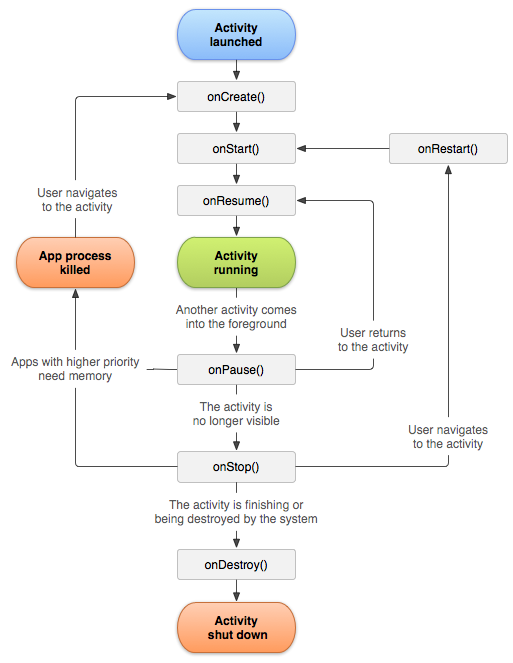
\includegraphics[width=12cm]{activity_lifecycle.png}
\caption{Ciclo di vita di una \emph{activity}}
\end{figure}


Una \emph{activity} implementa sei \emph{callbacks} fondamentali:

\begin{itemize}
    \item \texttt{onCreate}: viene chiamata quando il sistema crea l'activity, ed è all'interno di tale funzione che vengono effettuate le operazioni di inizializzazione che dovrebbero avvenire una sola volta durante l'intera vita dell'acivitiy;
    \item \texttt{onStart}: viene chiamata per rendere visibile l'activity all'utente, prima che essa venga eseguita in \emph{foreground} e diventi interattiva.
    \item \texttt{onResume}: viene chiamata ogni volta che l'attività deve essere eseguita in \emph{foreground}. L'attività rimane in questo stato finché non avviene un qualche evento che la porta in \emph{background}, come può essere una chiamata o l'apertura di un'altra applicazione.
    \item \texttt{onPause}: viene chiamata ogni volta che si presenta un evento che interrompe la normale esecuzione dell'activity. Questo non vuol dire che l'activity stia per essere distrutta, tantomeno che essa non sia più visibile dall'utente. Quando l'activity tornerà ad essere eseguita in \emph{foreground} verrà chiamata la funzione \texttt{onResume};
    \item \texttt{onStop}: viene chiamata quando l'activity non è più visibile dall'utente. L'activity in stato di \emph{stopped} è ancora presente in memoria. Da questo stato l'activity può tornare ad essere eseguita, e quindi verrà chiamata la funzione \texttt{onRestart}, oppure può essere distrutta, e quindi verrà chiamata la funzione \texttt{onDestroy};
    \item \texttt{onDestroy}: viene chiamata prima che l'activity venga distrutta, ed è lo stato finale del ciclo di vita dell'activity.
\end{itemize}
\hypertarget{fragment}{%
\subsection{Fragment}\label{fragment}}

Un Fragment rappresenta una porzione dell'interfaccia utente dell'applicazione. Esso definisce e gestisce il suo layout, ha un ciclo di vita proprio e può gestire i suoi eventi di input.

Un fragment non può tuttavia esistere da solo, ma deve essere inserito all'interno di un'activity o di un altro fragment.

I fragments rendono l'applicazione più modulare e riusabile, in quanto permettono di dividere la UI in più parti gestibili separatamente e riutilizzabili all'interno di diverse activities. \cite{fragments}

Dato che un fragment può esistere solo all'interno di una activity, il ciclo di vita di uno e dell'altra si innestano.

I cicli di vita del fragment quindi andranno di pari passo a quelli della activity in cui è inserito, e quindi il Fragment invocherà i metodi
\texttt{onCreate}, \texttt{onStart} e \texttt{onResume}. \cite{fragment-lifecycle} \cite{framents-lifecycle-2}

La classe fragment però possiede anche dei metodi propri, i più importanti sono:

\begin{itemize}
    \item \texttt{onAttach}: viene chiamato quando il Fragment viene aggiunto ad un \texttt{FragmentManager} ed è collegato all'activity ospite;
    \item \texttt{onCreateView}: viene chiamato per restituire la \texttt{View} in cui è presente il layout dell'interfaccia. Tra i parametri di input riceve un \texttt{LayoutInflater} la cui utilità è quella dell'eleborazione di un layout definito in un file .xml;
    \item \texttt{onActivityCreated}: in questo momento la creazione dell'activity è completa ed il fragment potrà interagire con essa;
    \item \texttt{onDestroyView}: indica la rimozione dell'interfaccia utente dal fragment, e prepara quest'ultimo allo scollegamento dall'activity;
    \item \texttt{onDetach}: viene chiamato quando il frammento viene rimosso dal \texttt{FragmentManager} e quindi scollegato dall'activity ospite.
\end{itemize}
\begin{figure}[H]
\centering
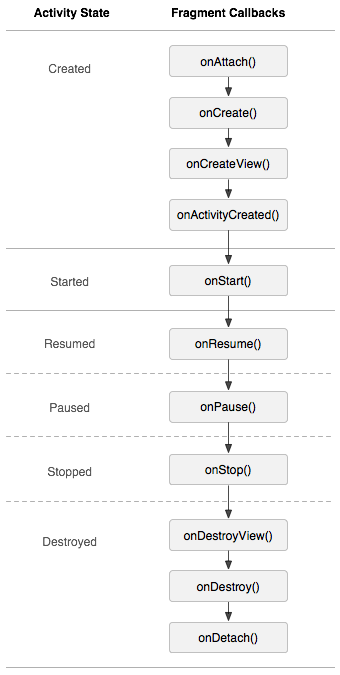
\includegraphics[width=8cm]{fragment_lifecycle.png}
\caption{Ciclo di vita di un \emph{fragment}}
\end{figure}

\hypertarget{intents}{%
\subsection{Intents}\label{intents}}

Un intent è un messaggio che viene usato da una componente dell'applicazione per richiedere un'azione da un'altra componente della stessa (o di un'altra) applicazione. \cite{intents}

Un intent può essere usato per:

\begin{itemize}
    \item Avviare un'activity;
    \item Avviare un \emph{service;}
    \item Inviare un messaggio in broadcast;
\end{itemize}
Esistono due tipi di \emph{intents}:

\begin{itemize}
    \item \textbf{Espliciti}: specificano quale componente verrà avviata per soddisfare l'intent. Un classico uso di un intent esplicito è per avviare un'activity a partire da un'altra activity;
    \item \textbf{Impliciti}: specificano solo un'azione generale, senza specificare la componente che andrà ad eseguire tale azione. Un esempio è quando si vuole effettuare un'azione tramite un'altra applicazione, e quindi si definisce l'azione, mostrando poi una finestra di dialogo in maniera tale che sia l'utente a scegliere con che applicazione eseguire tale azione.
\end{itemize}
\hypertarget{extras}{%
\subsubsection{Extras}\label{extras}}

Un intent porta con se delle coppie chiave-valore che possono essere inserite dalla componente che crea l'intent, e lette dalla componente che lo riceve.

\hypertarget{service}{%
\subsection{Service}\label{service}}

Un \emph{service} è una componente, non dotata di interfaccia grafica, all'interno di un'applicazione che permette di eseguire un operazione a lungo termine in \emph{background}. \cite{services}

Una volta eseguito, un \emph{service} può rimanere in esecuzione per un determinato lasso di tempo, anche in caso l'utente abbia cambiato applicazione.

Un \textit{service} può essere:
\begin{itemize}
    \item Foreground: esegue delle operazioni che possono essere notate dall'utente, ad esempio l'esecuzione di musica quando l'applicazione viene eseguita in background. Affinché il \textit{service} funzioni, l'applicazione deve mostrare un notifica durante tutta l'esecuzione del \textit{service};
    \item Background: esegue delle operazioni che non sono direttamente osservabili dall'utente, ad esempio la conversione da indirizzo sotto forma di stringa in coordinate.
\end{itemize}

\pagebreak


\hypertarget{gli-stati-dellutente}{%
\section{Gli stati dell'utente}\label{gli-stati-dellutente}}

L'applicazione implementa una macchina a stati finiti, il cui diagramma è mostrato di seguito.

\begin{figure}[H]
\centering
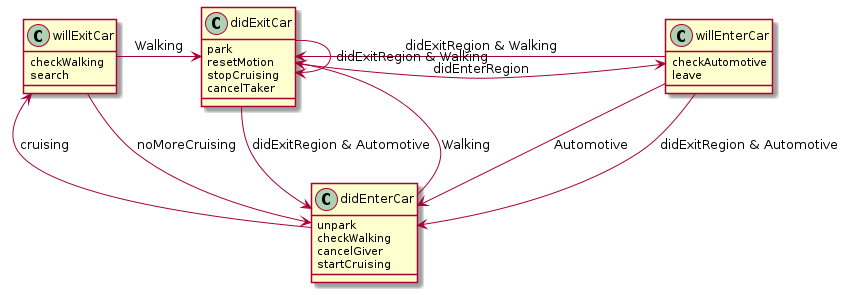
\includegraphics[width=12cm]{user_states.png}
\caption{Macchina a stati}
\end{figure}

Gli stati in cui può essere l'utente sono i seguenti:

\begin{itemize}
    \item \texttt{willExitCar}: l'utente ha parcheggiato e quindi sta per lasciare la macchina;
    \item \texttt{didExitCar}: l'utente ha parcheggiato dalla macchina ed è uscito da quest'ultima;
    \item \texttt{willEnterCar}: l'utente si sta avvicinando alla macchina a piedi e sta per entrare;
    \item \texttt{didEnterCar}: l'utente è entrato nella macchina parcheggiata e sta per uscire dal parcheggio.
\end{itemize}

\hypertarget{diagramma-uml-delle-classi}{%
\section{Diagramma UML delle classi}\label{diagramma-uml-delle-classi}}

Di seguito viene mostrato il diagramma UML delle delle classi, in cui vengono rappresentate le classi con cui il tirocinante ha interagito per l'implementazione delle funzionalità.

Le classi rappresentate da rettangoli a sfondo blu rappresentano le classi che sono state create durante il tirocinio, le altre rappresentano classi già esistenti nel progetto, che sono state inserite nel diagramma in quanto citate all'interno della relazione.

\begin{figure}[H]
\centering
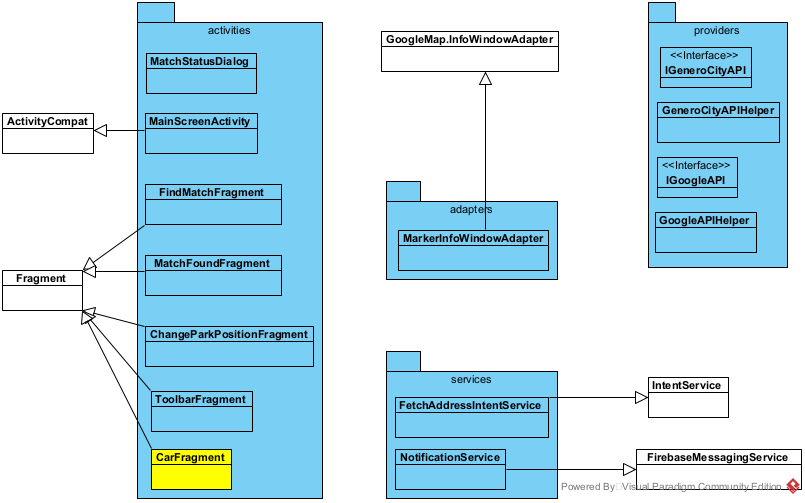
\includegraphics[width=12cm]{class_diagram.png}
\caption{Diagramma UML delle classi}
\end{figure}

\hypertarget{librerie-android-utilizzate}{%
\section{Librerie Android Utilizzate}\label{librerie-android-utilizzate}}

\hypertarget{retrofit}{%
\subsection{Retrofit}\label{retrofit}}

Retrofit è una libreria Java che permette di gestire in maniera semplice chiamate e risposte ad API REST.

La libreria Retrofit necessità l'implementazione di tre tipologie di classi:

\begin{itemize}
    \item Una classe per ogni oggetto che si vuole modellare, che verrà usata per la conversione da \texttt{json} ad oggetto java e viceversa;
    \item Un'interfaccia nella quale vengono definite le possibili API da chiamare;
    \item Una classe che implementa l'interfaccia definita nel punto precedente, ed in cui viene creato il Client Retrofit.
\end{itemize}
All'interno dell'interfaccia, ogni metodo rappresenta una possibile chiamata alle API. Vengono usate delle annotazioni del tipo
\texttt{@GET(”/me/”)} per definire l'endpoint della chiamata alle API ed il metodo HTTP. \cite{retrofit}

All'interno della classe definita nel terzo punto, viene costruito il Client nella seguente maniera

\begin{lstlisting} OkHttpClient client = httpClient.build(); 
Retrofit retrofit = new Retrofit.Builder()  
    .baseUrl(GCEnv.SERVER_URL)  
    .addConverterFactory(ScalarsConverterFactory.create())  
    .addConverterFactory(GsonConverterFactory.create(new GsonBuilder().excludeFieldsWithoutExposeAnnotation().create()))  
    .client(client) 
    .build();
return retrofit.create(IGeneroCityAPI.class);
\end{lstlisting}


\hypertarget{gson}{%
\subsection{Gson}\label{gson}}

\texttt{Gson} è una libreria Java (nel progetto integrata con Retrofit) che permette di convertire oggetti Java nella rappresentazione in oggetti \texttt{Json} e viceversa.

Tali oggetti Java modellano i vari elementi nel mondo reale trattati dal sistema. Gli oggetti rilevanti all'interno del lavoro svolto sono \texttt{Park} e \texttt{Match}. Visto che questi presentano un elevato numero di campi, di seguito verranno descritti quelli trattati maggiormente nel processo di sviluppo.

\hypertarget{park}{%
\subsubsection{Park}\label{park}}

Modella un parcheggio effettuato da un utente.

I campi più rilevanti sono:

\begin{itemize}
    \item \texttt{parktype}: indica il tipo di parcheggio, che può essere sconosciuto, a spina, parallelo o a pettine;
    \item \texttt{parkid}: intero che rappresenta il codice univoco del parcheggio;
    \item \texttt{parklat}: latitudine del parcheggio;
    \item \texttt{parklon}: longitudine del parcheggio;
    \item \texttt{starttime}: timestamp formattato come stringa che indica l'istante in cui l'utente ha parcheggiato;
    \item \texttt{endttime} timestamp formattato come stringa che indica l'istante in cui l'utente ha lasciato il parcheggio;
    \item \texttt{takerid}: codice univoco dell'utente che ha trovato il parcheggio tramite una ``ricerca posto''. Vale 0 se non esiste;
    \item \texttt{giverid}: codice univoco dell'utente che ha lasciato il posto tramite un ``lascia posto''. Vale 0 se non esiste.
\end{itemize}
\hypertarget{match}{%
\subsubsection{Match}\label{match}}

Modella un match, e presenta i seguenti campi:

\begin{itemize}
    \item \texttt{takerid}: codice univoco dell'utente Taker;
    \item \texttt{takercid}: codice univoco dell'auto con cui il Taker ha effettuato il match;
    \item \texttt{takerlat}: latitudine della posizione in cui il Taker intende trovare parcheggio;
    \item \texttt{takerlon}: longitudine della posizione in cui il Taker intende trovare parcheggio;
    \item \texttt{giverid}: codice univoco dell'utente giver
    \item \texttt{givercid}: codice univoco dell'auto con cui il Giver ha effettuato il match;
    \item \texttt{giverlat}: latitudine del parcheggio che il Giver intende lasciare;
    \item \texttt{giverlon}: longitudine del parcheggio che il Giver intende lasciare;
    \item \texttt{giverparkid}: codice univoco del parcheggio in cui è situata l'auto del giver;
    \item \texttt{parktype}: tipologia di parcheggio (si veda il campo omonimo in \texttt{park})
    \item \texttt{schedule}: timestamp che indica l'orario previsto in cui il Taker dovrebbe arrivare dal giver;
    \item \texttt{status}: indica lo stato del match nel momento corrente, il quale può assumere i seguenti valori:

 \begin{itemize}     \item  \texttt{waiting}: nel match è presente solamente il  Taker o il Giver in attesa che il sistema trovi un  utente con il ruolo opposto compatibile;     \item  \texttt{running}: il match è stato effettuato, e quindi sono  presenti sia Taker che Giver, ed è in corso di  esecuzione;     \item  \texttt{deleted}: il match, precedentemente in stato di  \texttt{waiting} è stato annullato dal Taker o dal Giver;     \item  \texttt{expired}: il match è scaduto perchè il Taker  non ha raggiunto la posizione del Giver entro 15 minuti;     \item  \texttt{success}: il match è stato completato con successo;     \item  \texttt{unsuccess-giver}: il match, precedentemente in  status di \texttt{running}, è stato annullato dal Giver;     \item  \texttt{unsuccess-taker}: il match, precedentemente in  status di \texttt{running}, è stato annullato dal Taker; \end{itemize}
    \item \texttt{updated}: timestamp formattato come stringa che indica l'istante in cui l'oggetto match ha ricevuto un aggiornamento di un qualche campo;
    \item \texttt{historyid}: codice univoco del match.
\end{itemize}

\hypertarget{progettazione}{%
\chapter{Progettazione}\label{progettazione}}

\hypertarget{architettura-del-sistema}{%
\section{Architettura del sistema}\label{architettura-del-sistema}}

L'architettura utilizzata da GeneroCity è del tipo \emph{client-server}.

\begin{figure}[H]
\centering
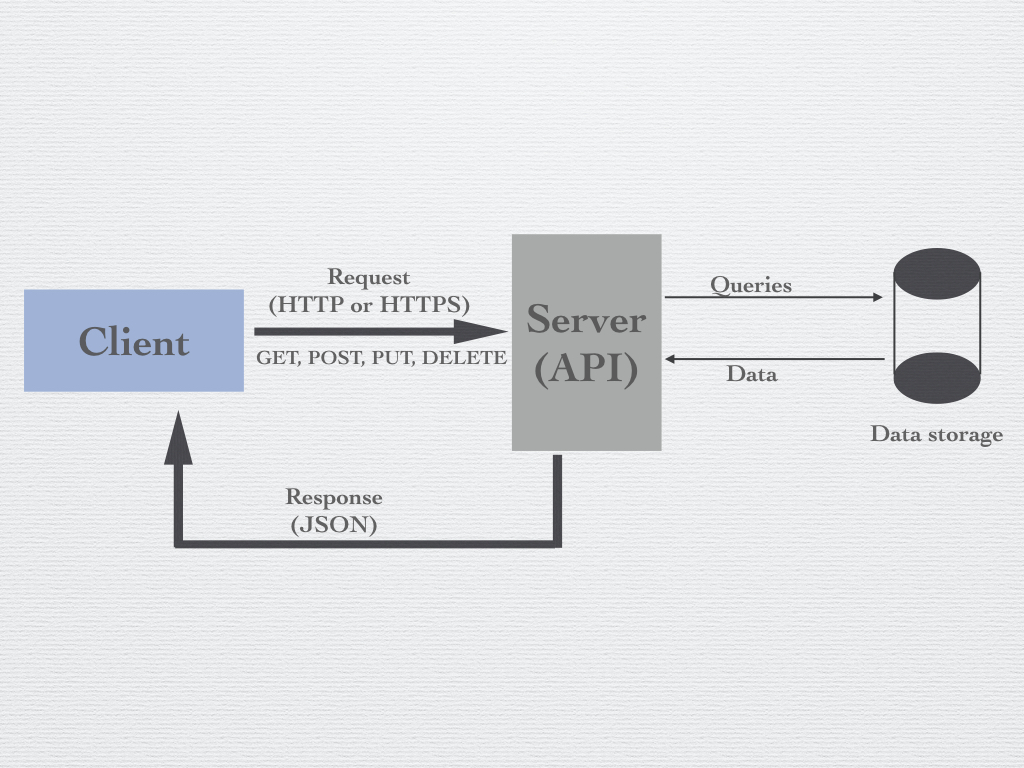
\includegraphics[width=12cm]{rest_architecture.jpg}
\caption{Diagramma di un'architettura client-server con API REST \cite{what-is-restful-api}}
\end{figure}


Il \emph{client}, ovvero il dispositivo Android dell'utente, comunica con il \emph{server} mediante delle chiamate alle API REST. La comunicazione permette al client l'accesso a delle risorse, ovvero a delle informazioni che il server decide di rendere disponibili per il client. \cite{rest-api-design}

La comunicazione avviene tramite il protocollo HTTP.

Una chiamata alle API REST contiene i seguenti elementi:

\begin{itemize}
    \item \textbf{\emph{Uniform Resource Identifier}} (\emph{URI}): indirizzo che indica dove trovare la risorsa su Internet;
    \item \textbf{Metodo} \texttt{HTTP}: indica l'operazione che bisogna effettuare con la risorsa indicata dall'URI. I principali metodi sono quattro:

 \begin{itemize}     \item  \texttt{GET}: permette di recuperare la risorsa, la quale verrà  mostrata in uno specifico formato (solitamente XML o JSON);     \item  \texttt{POST}: sostituisce la risorsa con un'altra risorsa,  solitamente indicata nel body;     \item  \texttt{PUT}: crea una nuova risorsa;     \item  \texttt{DELETE}: elimina la risorsa indicata. \end{itemize}
    \item \texttt{Header}: è una parte del messaggio che contiene delle informazioni chiave per entrambi il server ed il client. Tali informazioni possono essere ad esempio il formato della risposta, la chiave dell'API o l'indirizzo IP del server.
    \item \texttt{Body} (opzionale): viene utilizzato per inviare o ricevere ulteriori parti di dati.
\end{itemize}

\hypertarget{progettazione-ed-implementazione-di-funzionalituxe0-minori}{%
\section{Funzionalità minori}\label{progettazione-ed-implementazione-di-funzionalituxe0-minori}}

\hypertarget{implementazione-della-lista-dei-parcheggi}{%
\subsection{Implementazione della lista dei parcheggi}\label{implementazione-della-lista-dei-parcheggi}}

Lo scopo dell'implementazione dell'interfaccia di cui si andrà a parlare è quello di mostrare agli utenti uno storico dei parcheggi che sono stati effettuati.

Tali parcheggi vengono inseriti all'interno di una lista, implementata in Android mediante una \texttt{RecyclerView}, i cui i singoli elementi sono cliccabili.

Il click su un elemento che modella un singolo parcheggio porta ad una schermata contenente maggiori dettagli su tale parcheggio.

\begin{figure}[H]
\centering
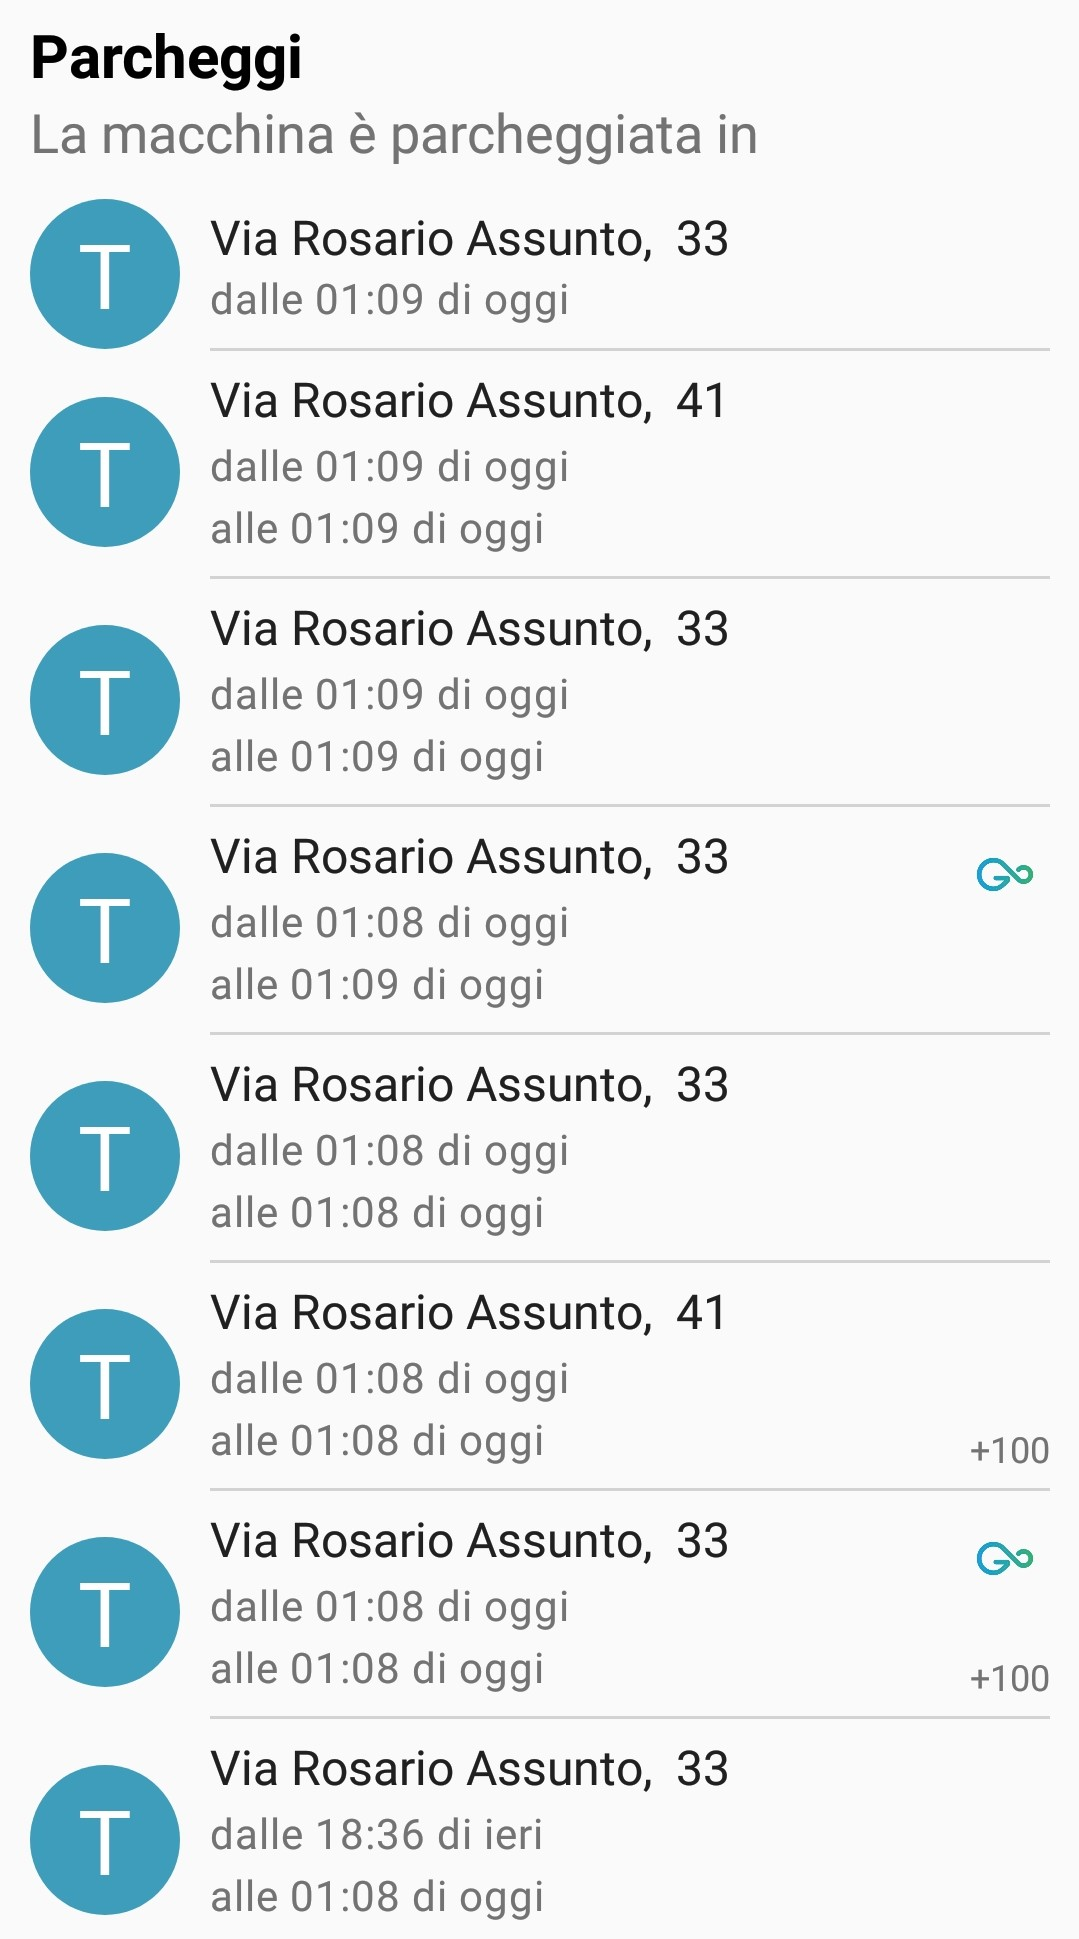
\includegraphics[width=6cm]{storico_parcheggi.jpg}
\caption{Storico parcheggi}
\label{storico-parcheggi}
\end{figure}

Negli elementi che compongono la lista sono presenti tre dati:

\begin{itemize}
    \item L'indirizzo, composto da via e civico, dove la macchina è stata parcheggiata
    \item L'orario e la data in cui la macchina è stata parcheggiata
    \item L'orario e la data in cui l'utente è uscito dal parcheggio
\end{itemize}
Il primo elemento della lista modella il parcheggio in cui l'auto dell'utente è correntemente situata. Essendo il parcheggio ancora in corso, non viene mostrato l'orario e la data in cui l'utente lo ha terminato. 

L'implementazione della lista dei parcheggi è stata sviluppata insieme ad altri due membri del team di sviluppo, a differenza delle altre funzioni di cui si parlerà nel resto della relazione.

\subsubsection{Paginazione dei risultati}

Prima dell'implementazione della funzionalità che verrà descritta, lo storico mostrava solamente gli ultimi 16 parcheggi effettuati dall'utente.

Questo avviene in quanto la chiamata alle API per ottenere la lista dei parcheggi effettuati con una macchina (\texttt{/car/\{cid\}/park/}) richiede opzionalmente come \emph{query parameter} un id del parcheggio.

Se questo parametro non viene inserito, l'API restituisce la lista degli ultimi 16 parcheggio effettuati, altrimenti restituisce la lista dei 16 parcheggi effettuati precedentemente al parcheggio passato come parametro.

Tramite questa logica è stato possibile paginare lo storico del parcheggi.

L'utente quando apre la schermata visualizza solo i 16 parcheggi più recenti. Quando effettua uno \emph{scroll} ed arriva in fondo alla pagina, l'app effettua una chiamata alle API inserendo come parametro l'ultimo parcheggio della lista, in maniera da recuperare i 16 parcheggi antecedenti all'ultimo parcheggio mostrato.

Durante la richiesta viene mostrata una progress bar, che viene rimossa quando i risultati sono disponibili.

Una volta che ciò accade, vengono inseriti ulteriori 16 parcheggi, o meno se i parcheggi totali sono inferiori, all'interno dello storico.

L'utente può continuare ad effettuare uno \emph{scroll} finché non visualizza tutti i parcheggi effettuati dalla macchina corrente.

\hypertarget{indicatori-di-scambio-nel-parcheggio}{%
\subsection{Indicatori di scambio nel parcheggio}\label{indicatori-di-scambio-nel-parcheggio}}

\begin{figure}[H]
\centering

\includegraphics[width=3cm]{images/gc-logo.png}
\caption{Logo di GeneroCity.}
\label{gc-logo}
\end{figure}

Aprendo lo storico dei parcheggi effettuati dall'utente, non era possibile capire a colpo d'occhio quali fossero i parcheggi effettuati tramite uno scambio con un altro utente, e quali fossero quelli effettuati senza uno scambio

Per ovviare a questa problematica, sono state inserite due icone alla destra di ogni elemento della lista dello storico dei parcheggi, che fanno capire all'utente la natura dello scambio (se presente). È possibile vedere una rappresentazione delle icone nella \autoref{storico-parcheggi}

L'icona presente in \autoref{gc-logo} è presente se il parcheggio è stato ottenuto mediante il completamento di un match; mentre il testo che indica "+100" è presente se il parcheggio è stato lasciato ad un utente mediante il completamento di un match. 

\pagebreak


\hypertarget{progettazione-del-sistema-di-scambio}{%
\section{Gestione dei matches}\label{progettazione-del-sistema-di-scambio}}

Nella seguente sezione verranno mostrate e documentate le interfacce che sono state realizzate ed il processo che ha portato alla loro realizzazione.

In particolare, sono state realizzate le schermate che permettono all'utente di:
\begin{itemize}      \item Comunicare al sistema l'intenzione di lasciare il posto ad un altro utente (diventare giver);      \item Chiedere al sistema di trovare un posto disponibile da occupare (diventare Taker);      \item Permettere di vedere se il sistema stia attualmente cercando un utente con ruolo opposto compatibile con cui scambiare il posto, ed eventualmente annullare tale ricerca;      \item Permettere di vedere informazioni utili circa il match in corso, come  la posizione del Taker e del Giver, il percorso tra il  Taker ed il Giver ed il tempo stimato di arrivo.
\end{itemize}
\hypertarget{cosuxe8-un-match}{%
\paragraph{Cos'è un match}\label{cosuxe8-un-match}}

Quando un utente parcheggiato comunica all'app di voler lasciare il posto, egli diventa un Giver.

Quando invece un utente comunica all'app di voler cercare un posto disponibile da occupare, diventa un Taker.

Quando un Taker ed un Giver sono compatibili, viene effettuato un \emph{match}. Quando si è all'interno di un match in corso, il Giver attende l'arrivo del Taker. Quando il
Taker raggiunge il Giver, quest'ultimo può lasciare il posto, che verrà occupato dal Taker. In tal caso il match viene completato con successo.

Il Taker ha un tempo di 15 minuti per raggiungere il Giver prima che il match venga annullato.

\hypertarget{struttura-delle-schermate}{%
\subsection{Struttura delle schermate}\label{struttura-delle-schermate}}

Le schermate che sono state progettate hanno tutte la medesima struttura, rappresentata nella \autoref{wireframe}.

\begin{figure}[H]
\centering
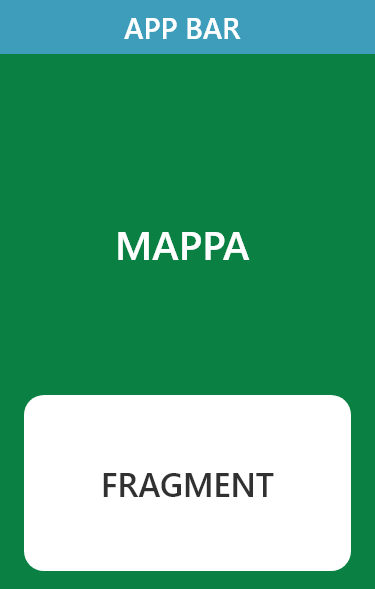
\includegraphics[width=6cm]{images/wireframe.png}
\caption{Wireframe delle schermate implementate.}
\label{wireframe}
\end{figure}

In alto è presente l'app bar, la quale contiene il nome dell'applicazione e dei pulsanti per effettuare delle azioni contestuali alla schermata in cui l'utente si trova.

Sottostante all'app bar è presente la mappa, ovvero un \texttt{Fragment} contenente una mappa fornita da Google su cui è possibile mostrare degli elementi.

Nella parte inferiore dello schermo è presente un \texttt{Fragment} che verrà sostituito a seconda della natura della schermata.

Il \texttt{Fragment} che viene mostrato all'apertura dell'applicazione è il \texttt{CarFragment} , già esistente all'inizio del tirocinio.

I metodi per effettuare le operazioni sui \texttt{Fragments} sono inseriti all'interno di una classe \texttt{FragmentUtility}.

Nei paragrafi successivi si parlerà proprio dei vari \texttt{Fragments} che sono stati sviluppati, e del modo in cui sono stati integrati all'interno del resto dell'interfaccia.

\hypertarget{toggle-per-registrare-e-rimuovere-un-parcheggio}{%
\subsection{Registrare e rimuovere un parcheggio}\label{toggle-per-registrare-e-rimuovere-un-parcheggio}}

L'applicazione registra un parcheggio quando una delle due condizioni si verifica:

\begin{itemize}
    \item L'utente preme il pulsante \texttt{PARCHEGGIATA} nella schermata principale;
    \item L'utente è in stato di \texttt{DidExitCar}.
\end{itemize}
L'applicazione rimuove un parcheggio quando una delle due condizioni si verifica:

\begin{itemize}
    \item L'utente preme il pulsante \texttt{IN USO} nella schermata principale;
    \item L'utente è in stato di \texttt{DidEnterCar}.
\end{itemize}
Il bottone per parcheggiare e rimuovere il parcheggio manualmente viene inserito in quanto il sistema potrebbe errare nella rilevazione automatica dello stato dell'utente (parcheggiato o non parcheggiato), e quindi all'utente viene data la possibilità di riallineare il sistema alla realtà, comunicando lo stato della macchina come ``parcheggiata'' o ``in uso'' mediante dei pulsanti dedicati.

\begin{figure}[H]
\centering
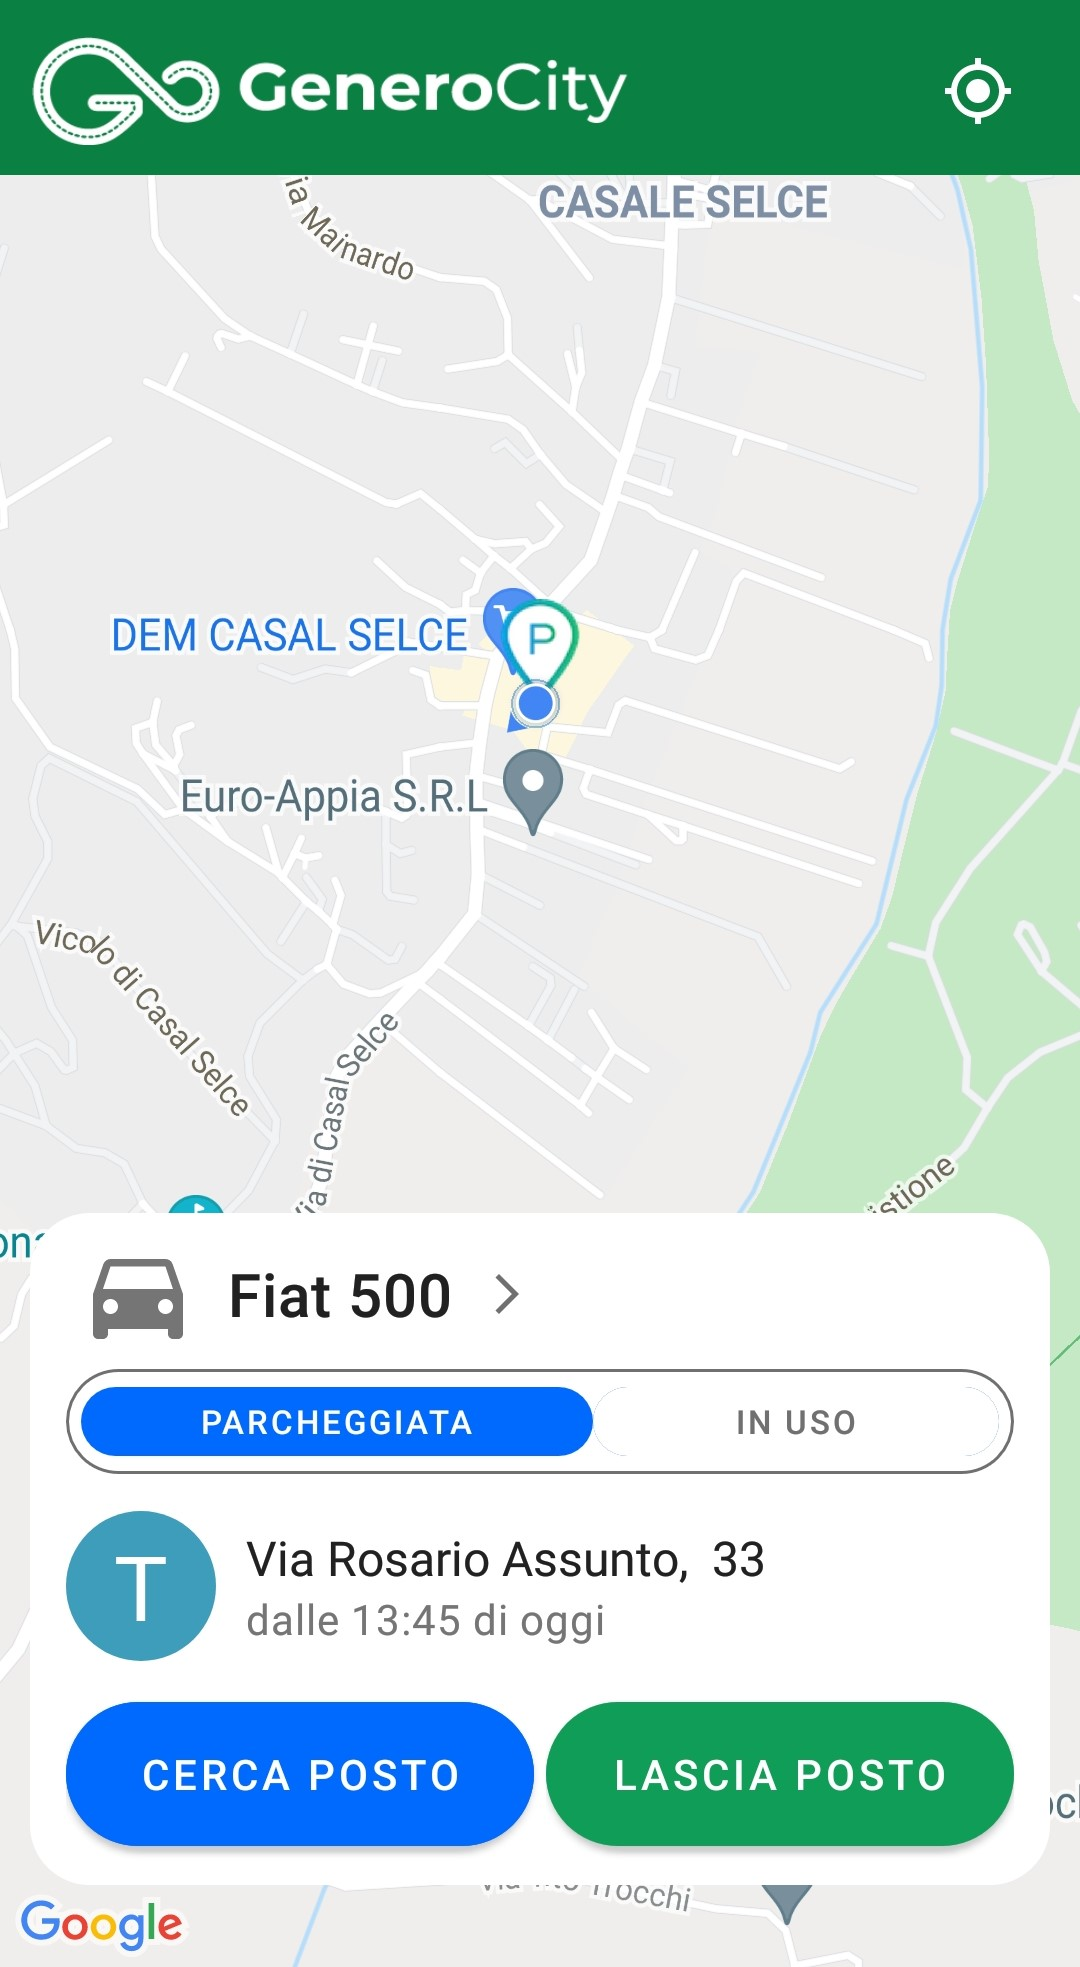
\includegraphics[width=6cm]{park_button_parked.jpg}
\caption{Interfaccia della pagina principale quando l'auto è parcheggiata.}
\end{figure}

In questo caso l'auto è parcheggiata e l'utente può premere sul pulsante \texttt{IN USO} per rimuovere tale parcheggio e comunicare all'applicazione che l'auto è attualmente in uso.

\begin{figure}[H]
\centering
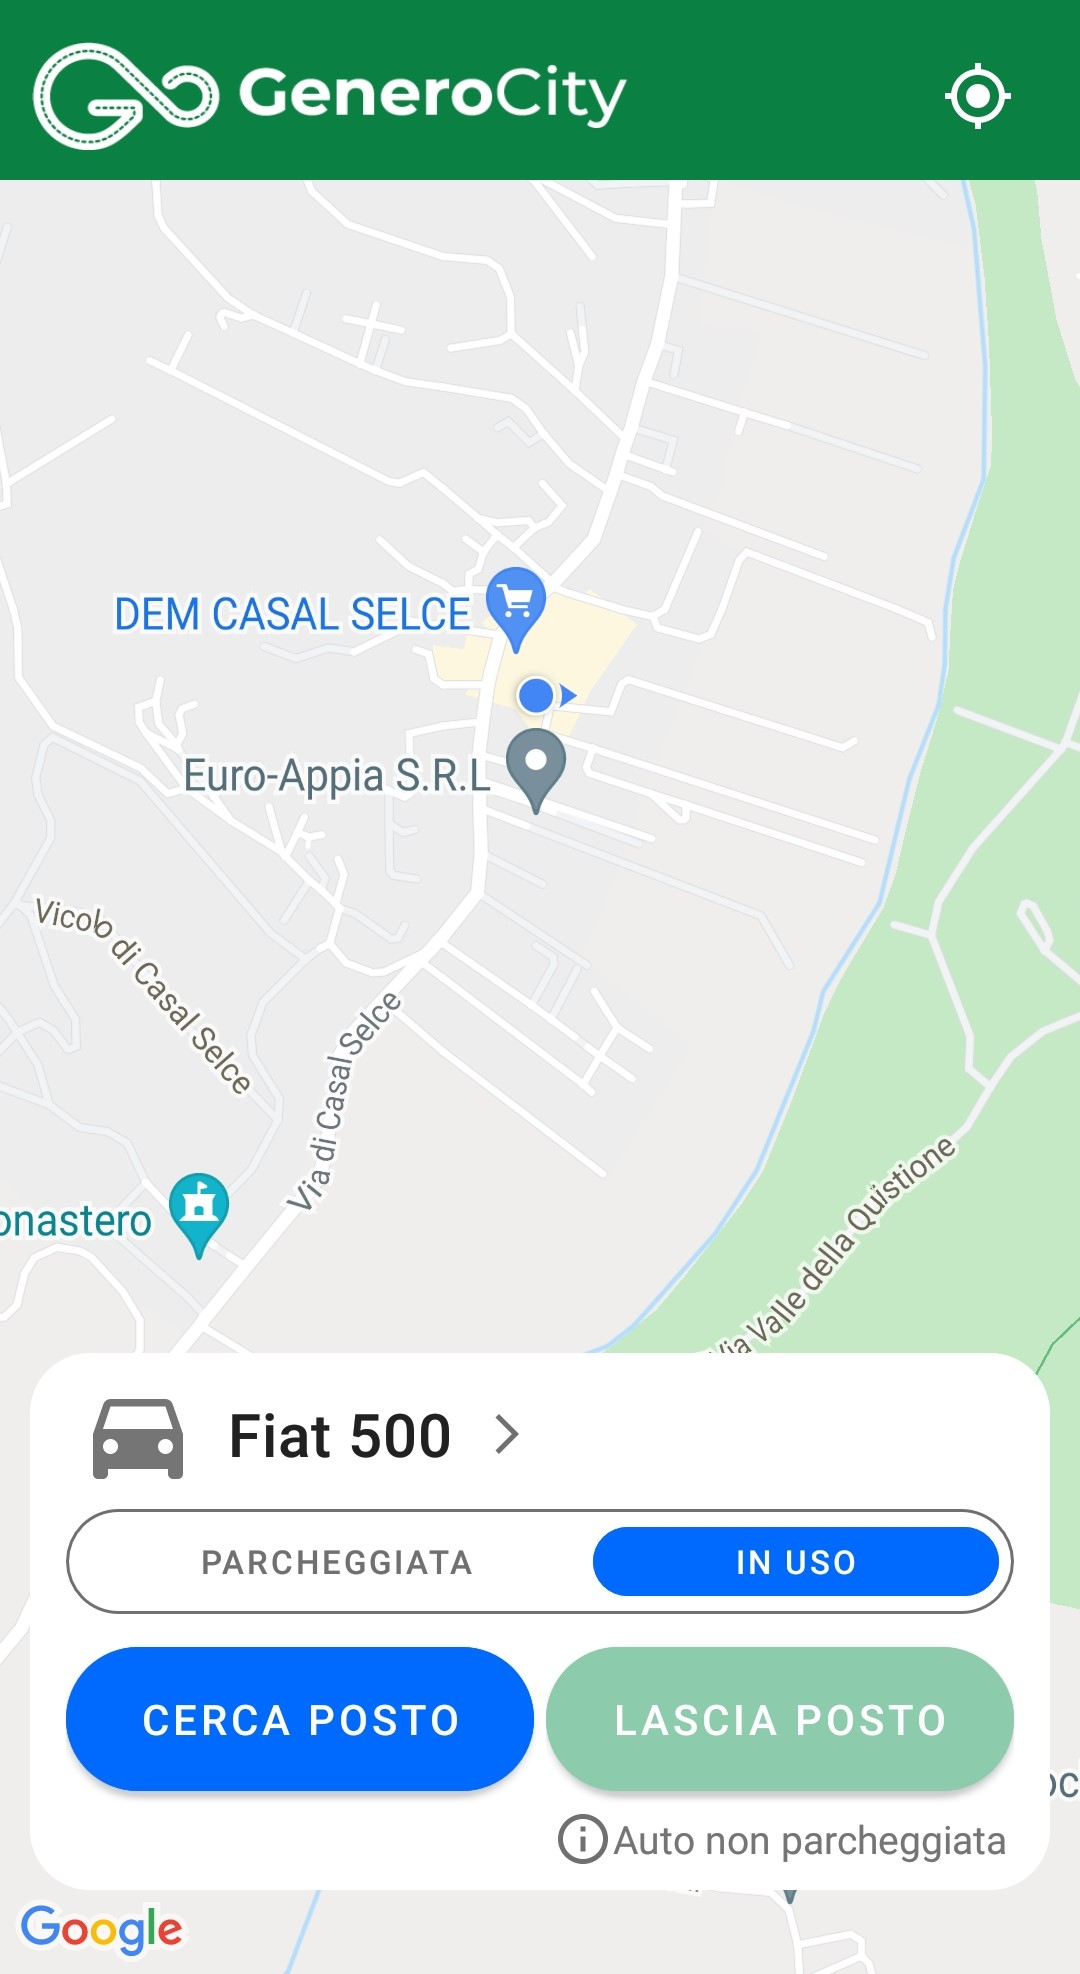
\includegraphics[width=6cm]{park_button_use.jpg}
\caption{Interfaccia della pagina principale quando l'auto è in uso.}
\end{figure}

In questo caso l'auto è in uso, ma l'utente può premere il pulsante \texttt{PARCHEGGIATA} per parcheggiare l'auto nella sua posizione attuale.

\hypertarget{test-effettuati}{%
\subsubsection{Test effettuati}\label{test-effettuati}}

Per verificare se ci fossero dei problemi legati all'usabilità dell'interfaccia, sono stati effettuati dei test sul campo con degli utenti.

Tali utenti sono stati inseriti in un'ipotetica situazione in cui il sistema segnalava che la loro macchina fosse in uso, quando in realtà questa era parcheggiata. Si è quindi chiesto loro di comunicare al sistema il fatto che l'auto fosse parcheggiata nel luogo in cui ora loro si trovavano.

Agli stessi utenti è stato effettuato anche il test inverso, e quindi è stato detto loro di comunicare al sistema che la macchina non era realmente parcheggiata in un luogo, ma che fosse attualmente in uso.

Tutti i test sono andati a buon fine e quindi si è concluso che l'interfaccia fosse utilizzabile in maniera corretta.

\hypertarget{interfaccia-per-ricerca-di-un-match}{%
\subsection{Ricerca di un match}\label{interfaccia-per-ricerca-di-un-match}}

La classe \texttt{FindMatchFragment} modella un \texttt{Fragment} che viene mostrato all'utente quando è in corso una ricerca, da parte del sistema, di un utente compatibile con cui effettuare uno scambio.

Si accede a tale schermata in tre modi:

\begin{itemize}
    \item Premendo il bottone ``cerca posto'' nella schermata inziale.
    \item Premendo il bottone ``lascia posto'' nella schermata iniziale.
    \item In caso di ripristino dello stato dell'\emph{activity} dopo che questa è stata chiusa.
\end{itemize}
Il \texttt{FindMatchFragment} rimpiazza sempre il \texttt{CarFragment}.

Per evitare duplicazione di codice, il \texttt{Fragment} utilizza solo un layout \texttt{xml} il quale viene modificato a tempo di esecuzione a seconda del ruolo dell'utente, in maniera da mostrare le informazioni utili al Taker o al giver.

La \emph{\texttt{view}} del \texttt{fragment} mostra all'utente i seguenti elementi:

\begin{itemize}
    \item Una \emph{label}, differente da Taker a Giver, che indica cosa l'utente stia cercando;
    \item Una \emph{progress bar} circolare che mostra all'utente che il processo di ricerca è in corso;
    \item Un bottone per annullare la ricerca.
\end{itemize}

\begin{figure}[H]
\centering
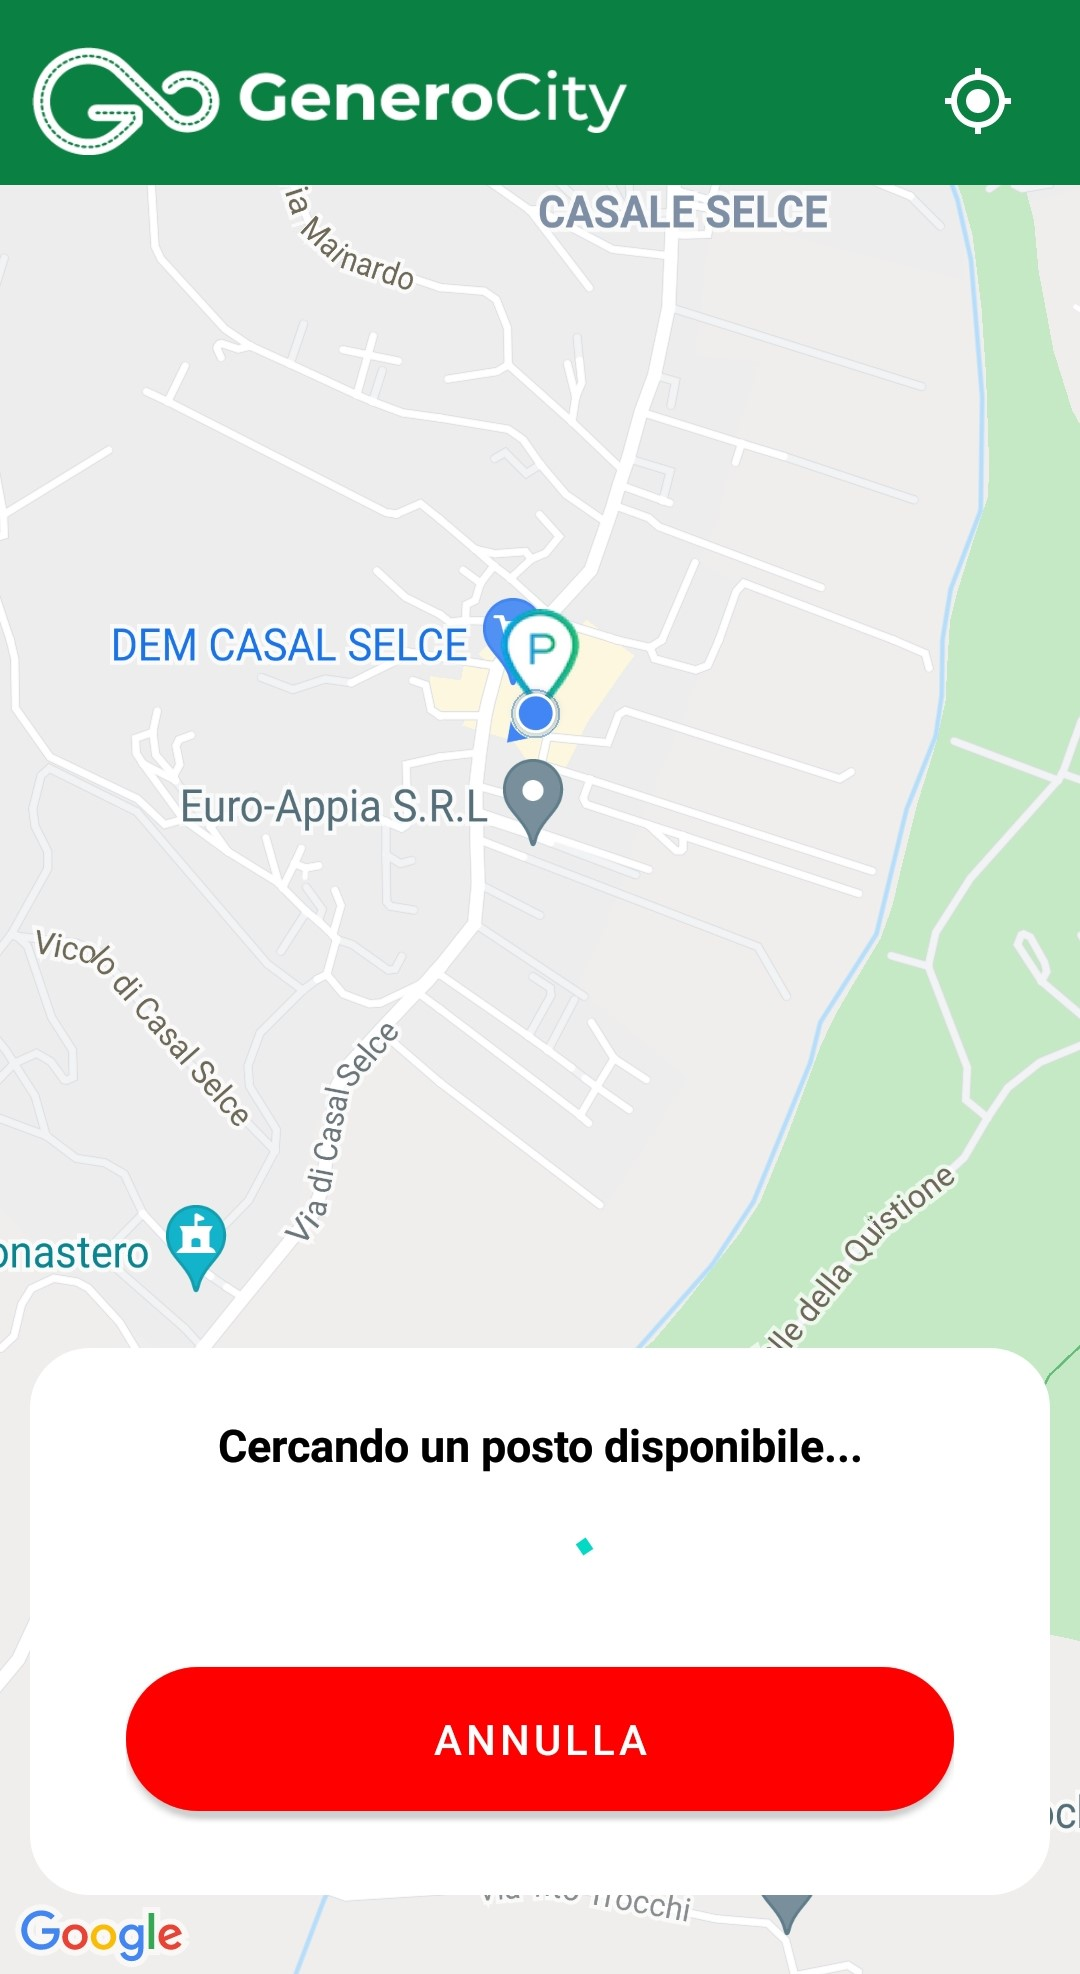
\includegraphics[width=6cm]{images/find_giver.jpg}
\caption{Interfaccia mostrata durante la ricerca di un Giver.}
\end{figure}

In caso del Taker, la label mostra la scritta ``Cercando un posto disponibile''


\begin{figure}[H]
\centering
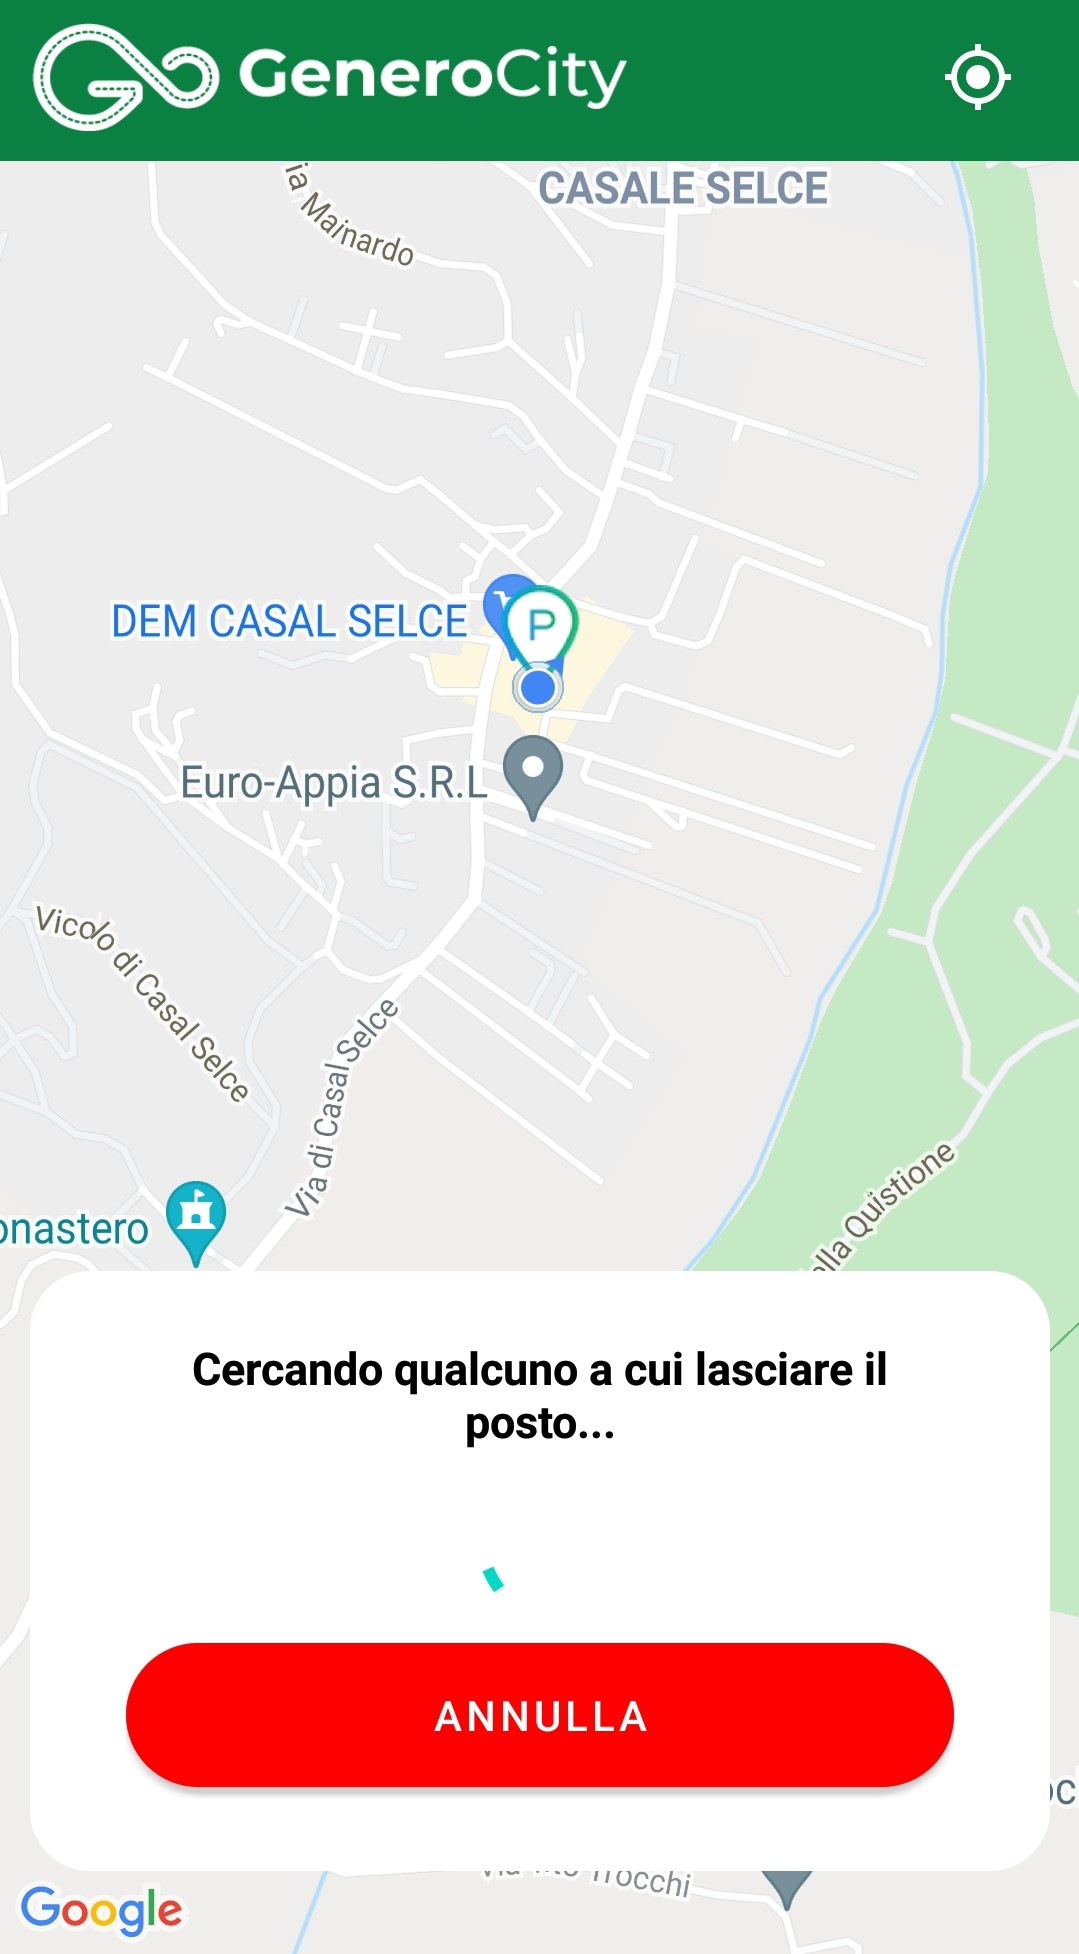
\includegraphics[width=6cm]{find_taker.jpg}
\caption{Interfaccia mostrata durante la ricerca di un Taker.}
\end{figure}

In caso del Giver, la label mostra la scritta ``Cercando qualcuno a cui lasciare il posto''.

\hypertarget{interfaccia-per-match-effettuato}{%
\subsection{Match effettuato}\label{interfaccia-per-match-effettuato}}

La classe \texttt{MatchFoundFragment} modella un \texttt{Fragment} che viene mostrato all'utente quando il sistema ha trovato un utente compatibile con cui effettuare uno scambio, e tale scambio è in corso di esecuzione.

La schermata può essere raggiunta dall'utente in tre modi:

\begin{itemize}
    \item Quando il sistema, per un utente nel ruolo di Taker, trova un utente Giver compatibile;
    \item Quando il sistema, per un utente nel ruolo di Giver, trova un utente Taker compatibile;
    \item In caso di ripristino dello stato dell'\emph{activity} dopo che questa è stata chiusa.
\end{itemize}
Nei primi due casi il \texttt{MatchFoundFragment} rimpiazza il
\texttt{FindMatchFragment}.

Nel terzo caso la UI si trova nella schermata iniziale, dove il Fragment mostrato sotto la mappa è il \texttt{CarFragment}. Per questo, quando la UI verrà ripristinata, il \texttt{MatchFoundFragment} ripristina il
\texttt{CarFragment}.

Anche qui è stato utilizzato un solo layout \texttt{xml} per evitare duplicazione di codice.


\begin{figure}[H]
\centering
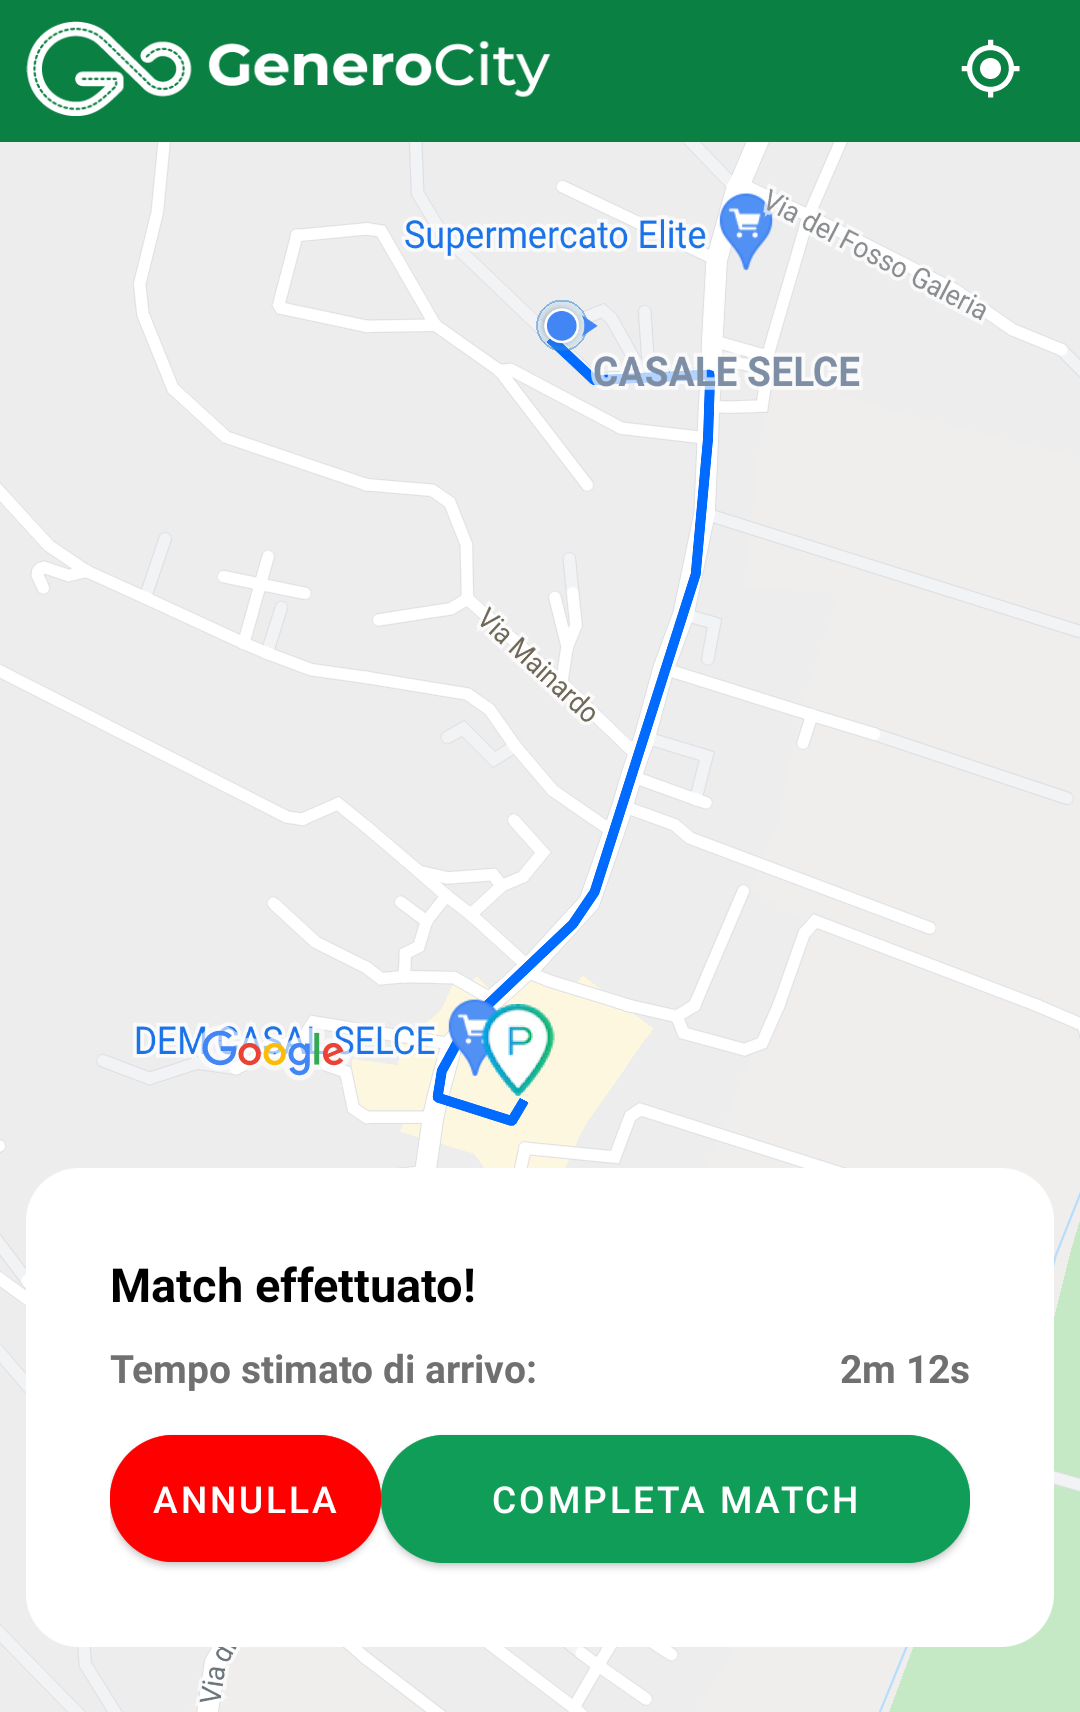
\includegraphics[width=6cm]{match_found_taker.png}
\caption{Interfaccia mostrata al Taker quando ha trovato un
Giver compatibile.}
\label{match-found-taker}
\end{figure}

Nel \texttt{Fragment} mostrato al Taker sono presenti quattro elementi:

\begin{itemize}
    \item Una \emph{label} che indica che un match è stato effettuato, e quindi che è presente un Giver compatibile pronto a cedere il posto auto;
    \item Una \emph{label} che indica il tempo stimato circa l'incontro tra i due utenti;
    \item Un bottone con dicitura ``Annulla'' che permette di annullare il match in corso. Sia il Taker che il Giver verranno portati nella pagina principale dell'applicazione;
    \item Un bottone con dicitura ``Completa match'' che permette di segnalare il match come confermato. Sia il Taker che il Giver verranno portati nella pagina principale dell'applicazione;
\end{itemize}
Nella mappa sono presenti tre elementi:

\begin{itemize}
    \item L'icona che rappresenta il punto in cui è parcheggiato il \emph{giver,} ovvero il punto che il Taker dovrà raggiungere;
    \item L'icona che rappresenta la posizione aggiornata del Taker, ovvero dell'utente che visualizza tale schermata;
    \item Il percorso che il Taker deve effettuare per arrivare dal giver;
\end{itemize}
\hypertarget{percorso-per-arrivare-dal-giver}{%
\subsubsection{Percorso per arrivare dal giver}\label{percorso-per-arrivare-dal-giver}}

Il percorso mostrato sulla mappa, che indica la strada che il Taker deve percorrere per arrivare dal Giver mediante un'automobile, è stato ottenuto mediante le \emph{Google Directions API}.

Il Taker, quando trova un Giver compatibile, effettua una chiamata alle Directions API all'url
\begin{verbatim}
    https://maps.googleapis.com/maps/api/directions/json
\end{verbatim}
in cui vengono inseriti come \textit{query parameters}, i seguenti campi:
\begin{itemize}
    \item \texttt{origin}: le coordinate (o indirizzo) del punto d'origine, ovvero l'attuale posizione del Taker;
    \item \texttt{destination}: le coordinate (o indirizzo) del punto destinazione, ovvero la posizione del Giver;
    \item \texttt{key}: la chiave per poter utilizzare le API.
\end{itemize}

Tale chiamata ritorna un oggetto json in cui sarà presente, in aggiunta ad altre informazioni, una codifica delle \texttt{Polylines} da inserire sulla mappa per mostrare il percorso tra i due punti.

Una \texttt{Polyline} è un segmento che mostra sulla mappa il collegamento tra due punti. La serie di \texttt{Polylines} che deve essere mostrata viene codificata da un algoritmo.
\begin{lstlisting}[caption=Lista di \texttt{Polylines} codificata]
    kox~Fq_kjALDGb@_@E]MMG]]qAuBq@eAY_@OOe@SqC}@yC}@gC}@o@KcGQqCIc@Ia
    A]aGsC}E{BeBw@oAg@UCQYg@c@c@g@[g@ESAwA@aA?kCLsCHiAFQ[k@W_@W_@c@}@
    _@aAs@eCWeBMe@GMaBgBeC}Be@]{A{@}@s@i@UiDeAeAO]Oc@WN{CJw@Z}@Ve@pAc
    BJ[Da@AoBHm@d@}Ab@}@lAmBb@m@SQMAe@Fs@Ca@?y@R}@f@yAlA[NqBh@sB`AQ@W
    ID_@@SFSFI\\OLQHg@?UG[u@wAO]UkAQg@]c@o@k@oBkAq@e@SWk@}@{@{BMw@PoF
    BgA?{@Es@CYG]u@G
\end{lstlisting}
 Il messaggio viene decodificato in un vettore di oggetti \texttt{LatLng}, che verranno utilizzati per costruire le varie \texttt{Polylines} sulla mappa, che nell'insieme formeranno il percorso mostrato in \autoref{match-found-taker}. 

\begin{figure}[H]
\centering
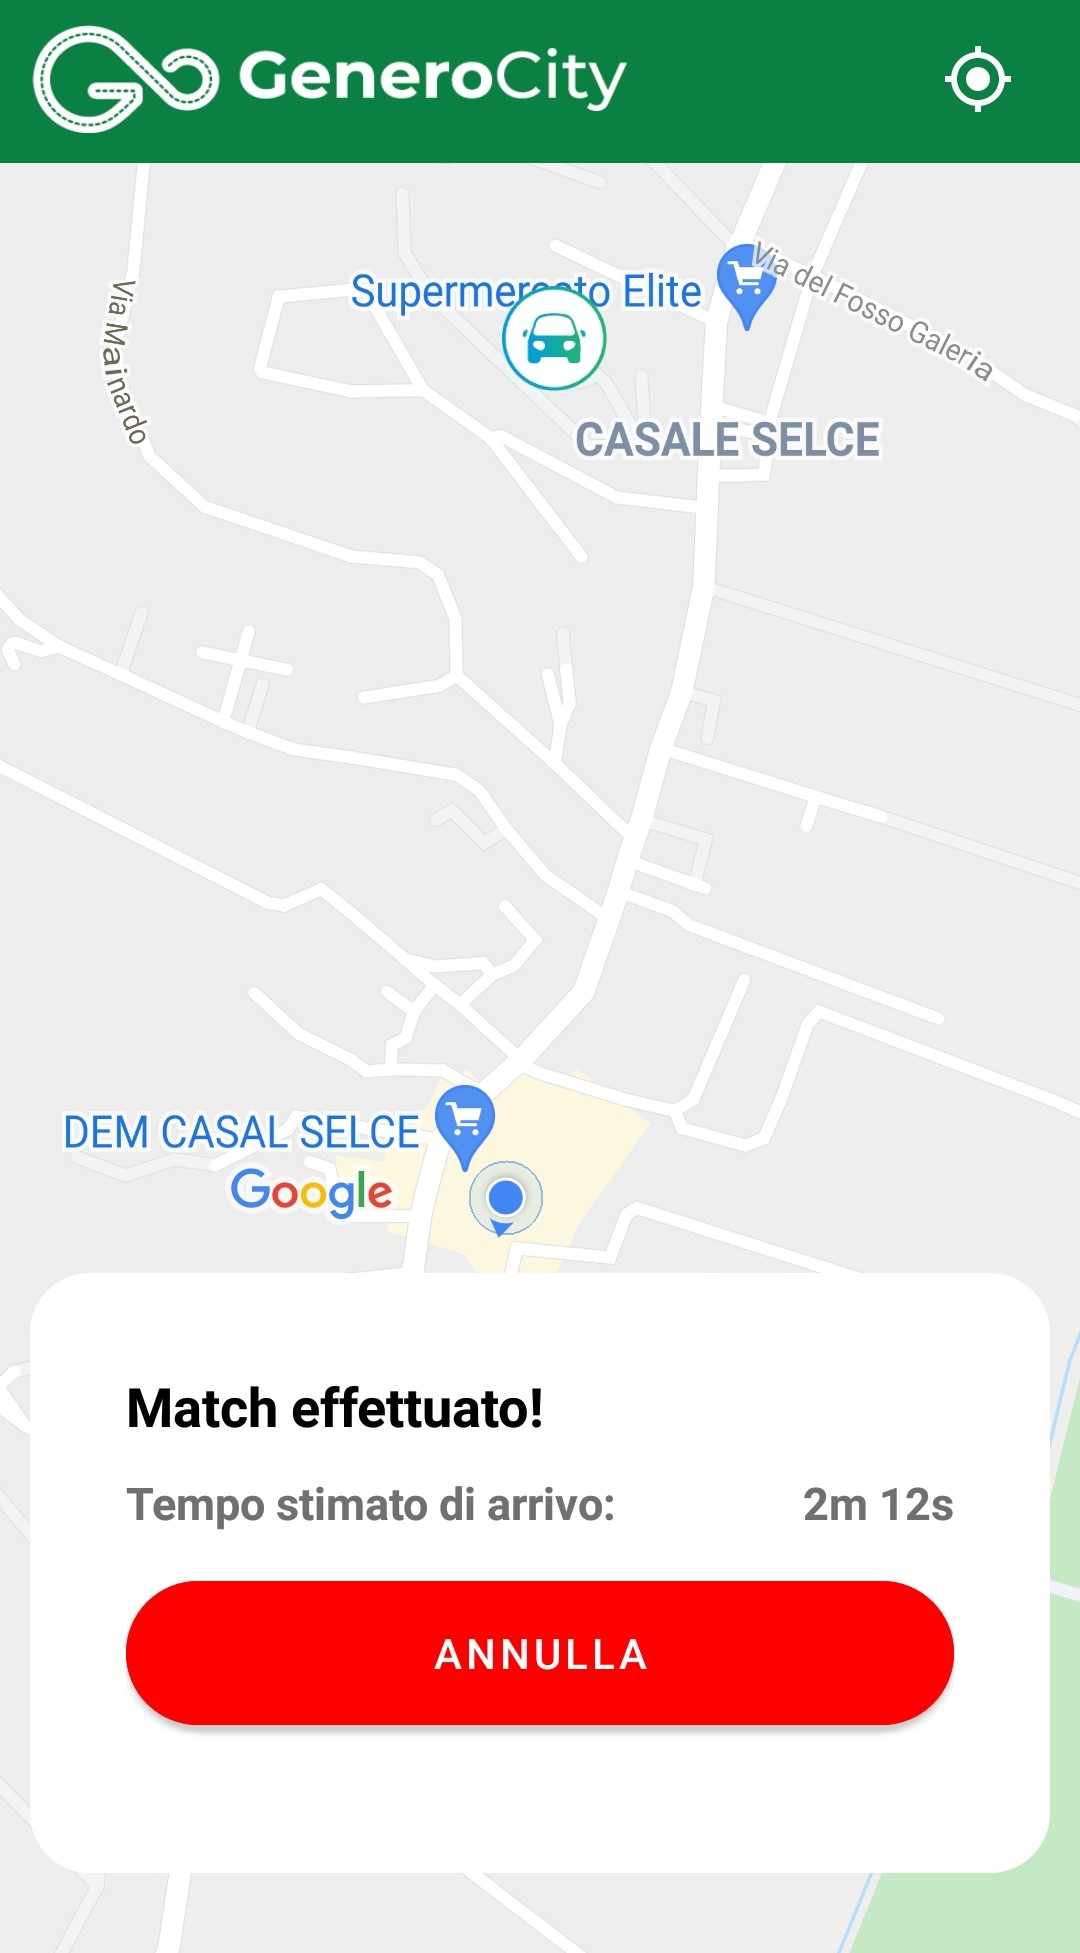
\includegraphics[width=6cm]{match_found_giver.jpg}
\caption{Interfaccia mostrata al Giver quando ha trovato un
Taker compatibile.}
\end{figure}


Per quanto riguarda il \texttt{Fragment} mostrato al Giver, sono presenti tre elementi:

\begin{itemize}
    \item Una \emph{label} che indica che un match è stato effettuato, e quindi che è presente un Taker compatibile a cui cedere il posto;
    \item Una \emph{label} che indica il tempo stimato circa l'incontro tra i due utenti;
    \item Un bottone con dicitura ``Annulla'' che permette di annullare il match in corso.
\end{itemize}
Nella mappa è presente il \textit{marker} che rappresenta la posizione, aggiornata in tempo reale, del Taker.

\hypertarget{aggiornamento-della-posizione-del-taker}{%
\subsubsection{Aggiornamento della posizione del taker}\label{aggiornamento-della-posizione-del-taker}}

Quando il Taker comincerà a guidare dirigendosi verso il
Giver, quest'ultimo vedrà sull'interfaccia il \emph{marker} che rappresenta la posizione del Taker muoversi in tempo reale.

Il risultato viene raggiunto nella seguente maniera:

\begin{enumerate}      
    \item Siano T e G rispettivamente il Taker ed il Giver all'interno di un match in stato Running;      
    \item Il client di T effettua, ogni \texttt{5000ms}, una chiamata alle API con endpoint \texttt{"/car/\{cid\}/position"} dove \texttt{\{cid\}} è il codice univoco dell'auto con cui il Taker vuole parcheggiare. La chiamata alle API ha un metodo \texttt{HTTP POST}, e richiede nel \texttt{body} un oggetto \texttt{json} con le informazioni relative alla posizione da inviare, che verranno documentate in dettaglio nella \autoref{invio-periodico-posizione-taker}.      
    \item Il server, alla ricezione di tale chiamata API, invia una notifica push al client del Giver, del tipo: 
        \begin{verbatim}  
        {x-gc-category:TAKERPOSITION, lat:42.2412, lon:12.4253, eta:2674}  
        \end{verbatim}      
    \item Il client di G, alla ricezione di ogni notifica push, estrae la nuova posizione di T ed aggiorna il rispettivo marker sulla mappa tramite un'animazione della durata di \texttt{5000ms}. 
\end{enumerate}

\hypertarget{tempo-previsto-per-larrivo-del-taker}{%
\subsubsection{Tempo previsto per l'incontro dei due utenti}\label{tempo-previsto-per-larrivo-del-taker}}

Su entrambe le interfacce viene mostrata l'informazione relativa al tempo rimanente stimato prima che i due utenti si incontrino.

Il Taker, immediatamente prima di effettuare una chiamata alle API per comunicare la posizione aggiornata al server, come visto nel paragrafo precedente, effettua una chiamata alle \emph{DistanceMatrix} Google APIs, all'url
\begin{verbatim}
    https://maps.googleapis.com/maps/api/distancematrix/json
\end{verbatim}
in cui vengono inseriti, come \textit{query parameters} i seguenti valori:
\begin{itemize}
    \item \texttt{origins}: le coordinate del punto d'origine, ovvero l'attuale posizione del Taker;
    \item \texttt{destinations}: le coordinate del punto destinazione, ovvero la posizione del Giver;
    \item \texttt{departure-time}: l'istante di partenza, impostato sempre su \texttt{now};
    \item \texttt{key}: la chiave per poter utilizzare le API.
\end{itemize}

Nell'oggetto json che il server manderà nel \texttt{body} della risposta alla chiamata API, sono presenti tre valori:
\begin{enumerate}
    \item Un valore che indica la distanza percorribile su strada, in metri, tra i due punti;
    \item Un valore che indica la durata del viaggio, in secondi, senza considerare il traffico;
    \item Un valore che indica la durata del viaggio, in secondi, considerando il traffico.
\end{enumerate}

Viene preso in considerazione solo il terzo valore che, una volta ottenuto, viene mostrato sull'interfaccia del Taker. Quando il Taker, immediatamente dopo, effettua la chiamata per aggiornate la posizione (\autoref{aggiornamento-della-posizione-del-taker}), inserisce tale valore nel campo \texttt{eta} all'interno del \texttt{body} della richiesta. 

Il Giver, alla ricezione della notifica vista in \autoref{aggiornamento-della-posizione-del-taker}, formatta il valore e lo inserisce nella sua interfaccia. 

\hypertarget{annullamento-di-un-match}{%
\subsection{Annullamento di un match}\label{annullamento-di-un-match}}

Un match, che sia in fase di ricerca o in corso, può essere annullato dalla parte di entrambi gli utenti coinvolti, mediante la pressione del bottone ``Annulla''.

\begin{figure}[H]
\centering
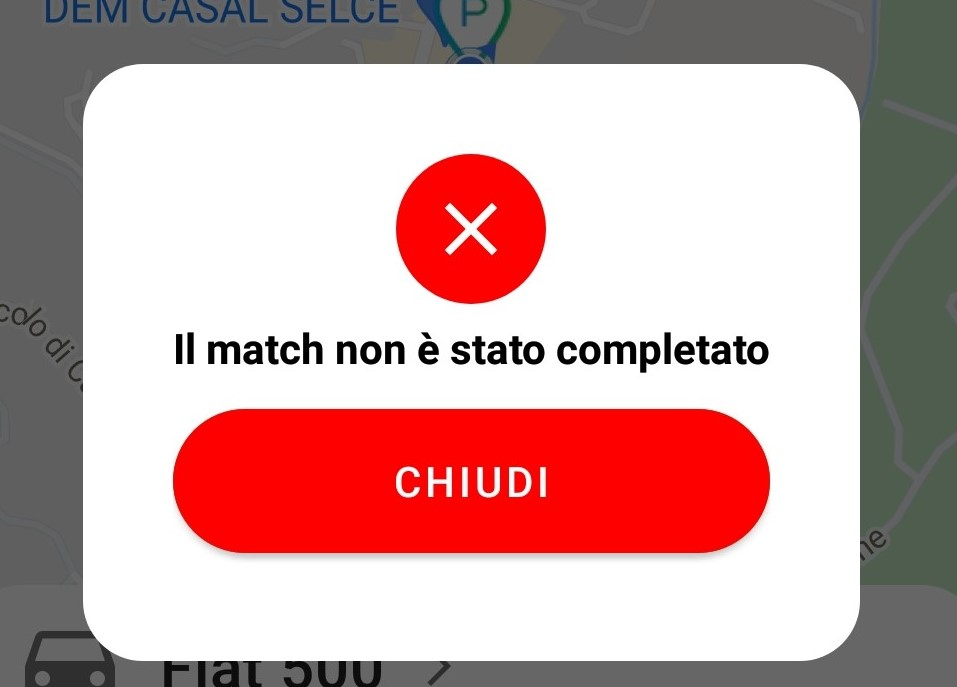
\includegraphics[width=6cm]{Dialog_match_non_completato.jpg}
\caption{Messaggio mostrato in caso il match non sia andato a buon
\label{Dialog_match_non_completato} fine.}
\end{figure}

\hypertarget{annullamento-di-un-match-in-fase-di-ricerca}{%
\subsubsection{Annullamento di un match in fase di ricerca}\label{annullamento-di-un-match-in-fase-di-ricerca}}

In caso di annullamento di un match in fase di ricerca, l'utente viene riportato alla schermata iniziale e viene mostrato una
\texttt{DialogWindow} (\autoref{Dialog_match_non_completato}) che comunica all'utente il corretto annullamento del match.

\hypertarget{annullamento-di-un-match-in-corso}{%
\subsubsection{Annullamento di un match in corso}\label{annullamento-di-un-match-in-corso}}

Visto che un match in corso comprende due utenti, l'annullamento da parte di un utente implica che il match venga annullato anche per il secondo utente.

Durante tutta la vita del frammento \texttt{MatchFoundFragment}, ovvero durante tutto il tempo in cui gli utenti sono all'interno di un match, un frammento di codice viene eseguito ogni 2 secondi, il cui scopo è quello di controllare se l'utente sia ancora in un match o meno. Questo avviene mediante una chiamata alle API.

Il flow dell'applicazione è quindi il seguente:

\begin{enumerate}
    \item Siano T e G rispettivamente un Taker ed un Giver all'interno di un match
    \item T annulla il match premendo sul pulsante ``Annulla'';
    \item T viene riportato alla pagina principale e gli viene mostrata la \emph{\texttt{DialogWindow}} che mostra i corretto annullamento del match (\autoref{Dialog_match_non_completato});
    \item Al più 2 secondi dopo dall'annullamento del match da parte di T, il codice che controlla lo stato del match riconosce che l'utente G non è più all'interno di un match;
    \item G viene riportato alla pagina principale e gli viene mostrata la medesima schermata di corretto annullamento del match.
\end{enumerate}

\hypertarget{completamento-di-un-match}{%
\subsection{Completamento di un match}\label{completamento-di-un-match}}

Un match può essere completato solamente se è in corso, e tale azione può essere effettuata solamente dal Taker, mediante la pressione del pulsante ``Completa'' nel \texttt{MatchFoundFragment}.

Il flow dell'applicazione è il seguente:

\begin{enumerate}

    \item Siano T e G rispettivamente un Taker ed un Giver all'interno di un match;
    \item T completa il match premendo sul pulsante ``Completa''';
    \item T viene riportato alla pagina principale e gli viene mostrata la \emph{\texttt{DialogWindow}} che mostra il corretto completamento del match (\autoref{Dialogo_match_completato});
    \item Al più 2 secondi dopo dall'annullamento del match da parte di T, il codice che controlla lo stato del match riconosce che il match che comprende G è stato completato;
    \item G viene riportato alla pagina principale e gli viene mostrata la \emph{\texttt{DialogWindow}} che mostra il corretto completamento del match (\autoref{Dialogo_match_completato};
\end{enumerate}

\begin{figure}[H]
\centering
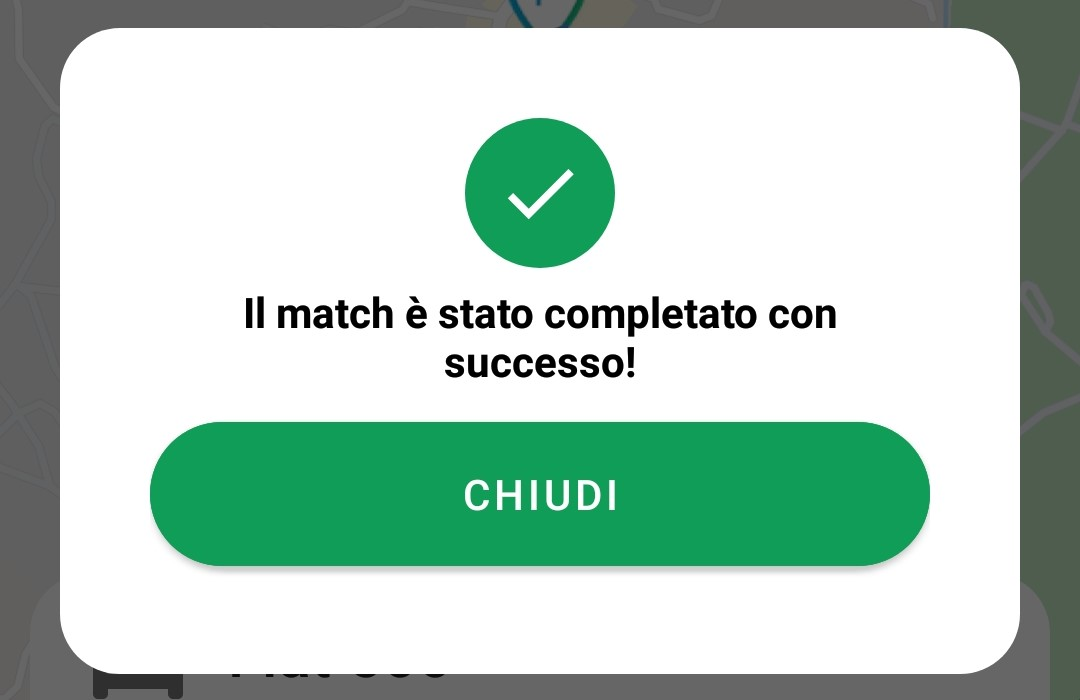
\includegraphics[width=6cm]{Dialogo_match_completato.jpg}
\caption{Messaggio mostrato in caso il match sia stato completato con successo.}
\label{Dialogo_match_completato}
\end{figure}

\hypertarget{modificare-posizione-parcheggio}{%
\section{Modifica posizione parcheggio}\label{modificare-posizione-parcheggio}}

Nello stato dell'applicazione prima dell'implementazione della modifica di cui si andrà a parlare, per l'utente non era possibile modificare la posizione di un parcheggio effettuato precedentemente.

\hypertarget{prima-iterazione}{%
\subsection{Prima iterazione}\label{prima-iterazione}}

\hypertarget{info-window}{%
\subsubsection{Info Window}\label{info-window}}

La \texttt{InfoWindow} è l'elemento che appare quando si clicca sopra un
\emph{marker} all'interno di una mappa. Tale elemento può essere personalizzato a piacere in maniera da contenere le informazioni che possono risultare più utili all'utente. Viene quindi aggiunta una funzionalità che permette all'utente di modificare la posizione del parcheggio in cui l'auto è attualmente parcheggiata. 

\begin{figure}[H]
\centering
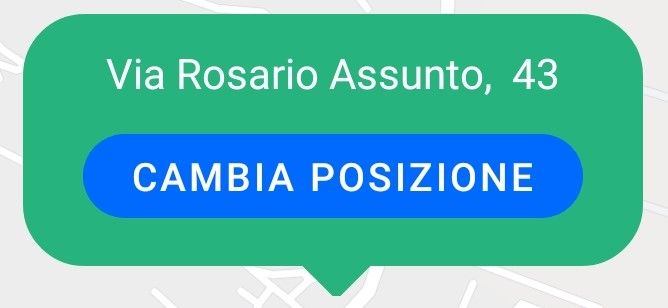
\includegraphics[width=6cm]{CustomInfoWindowCut.jpg}
\caption{La \texttt{InfoWindow} relativa al marker del parcheggio}
\label{info-window}
\end{figure}

In tale elemento sono presenti tre elementi:

\begin{itemize}
    \item L'indirizzo in cui è situato il \emph{marker};
    \item La distanza che separa la posizione del marker dalla posizione attuale dell'utente;
    \item Un pulsante che permette di modificare la posizione del \emph{marker};
\end{itemize}
\hypertarget{ui-per-la-modifica-del-parcheggio}{%
\subsubsection{UI per la modifica del parcheggio}\label{ui-per-la-modifica-del-parcheggio}}

\begin{figure}[H]
\centering
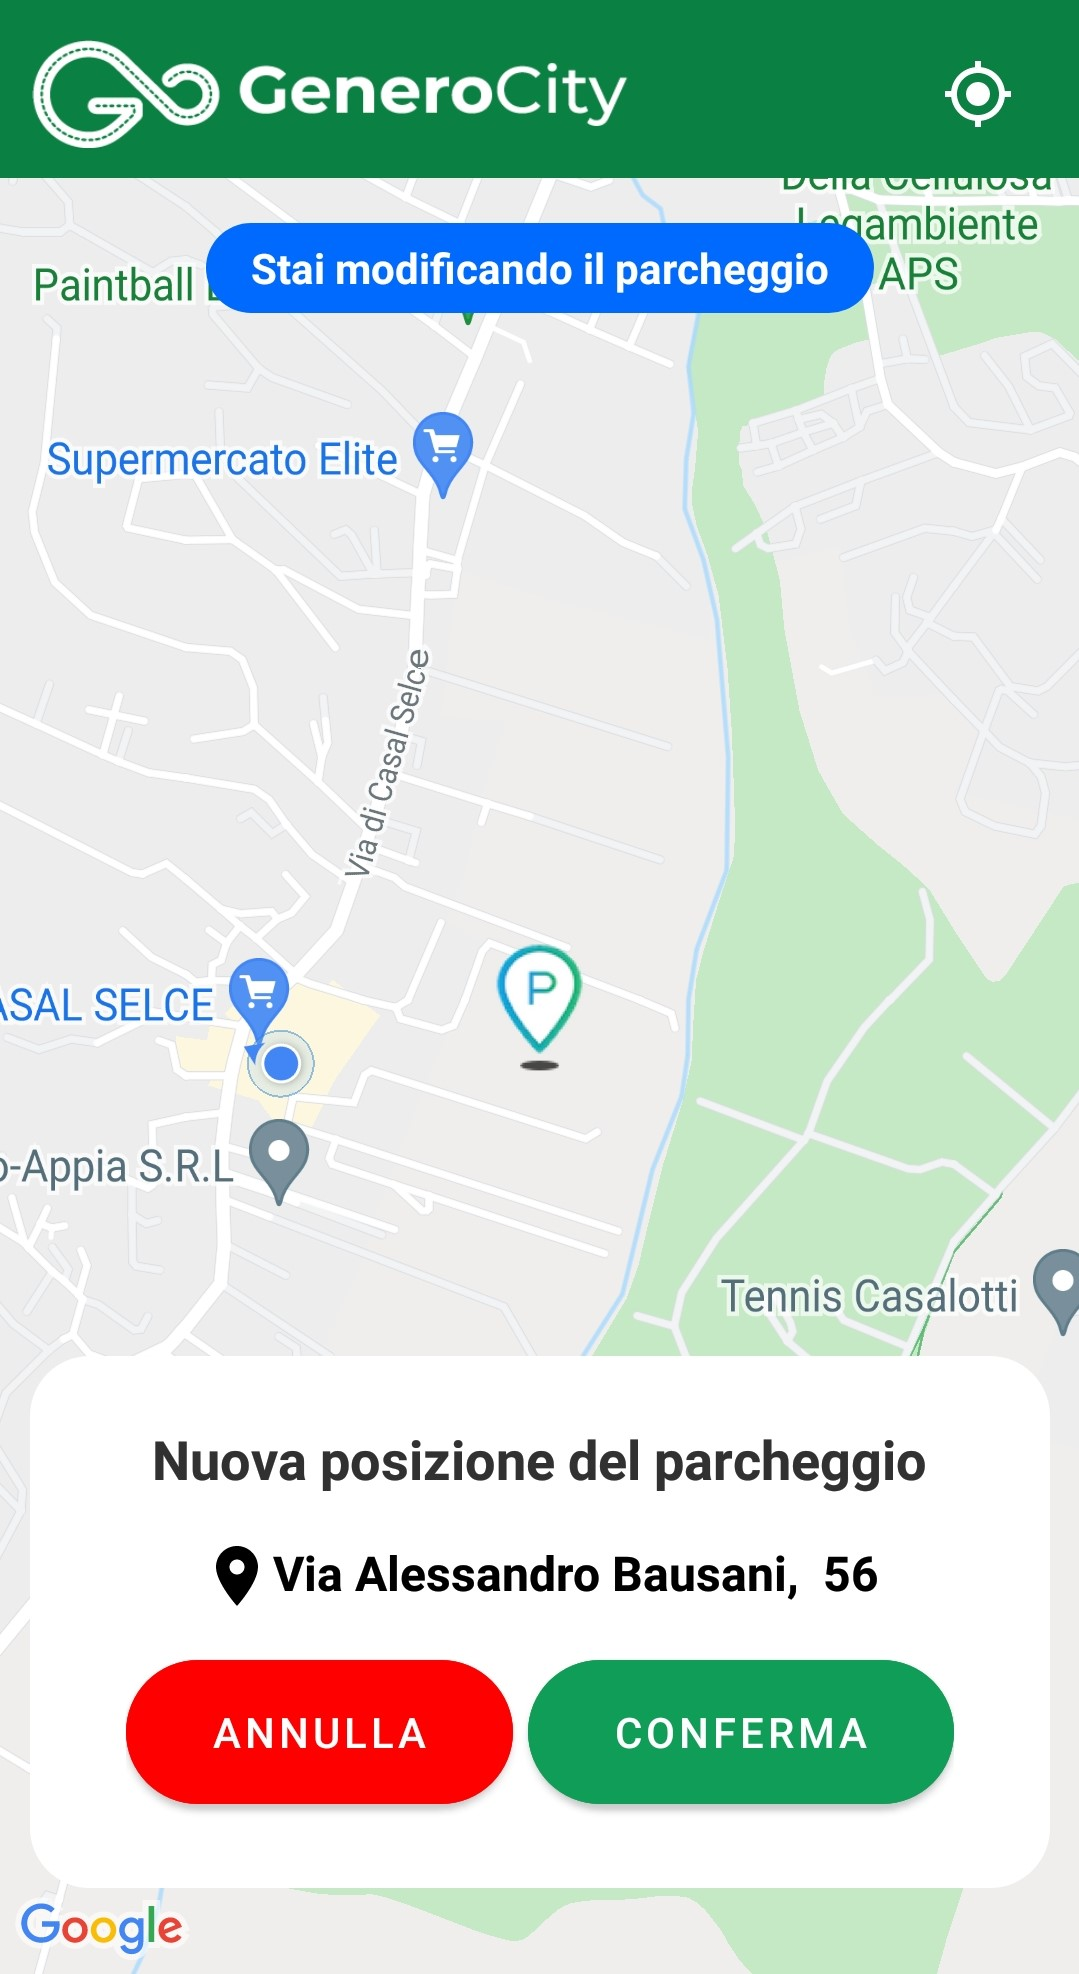
\includegraphics[width=6cm]{EditMode.jpg}
\caption{Prima iterazione della schermata per la modifica del parcheggio.}
\end{figure}

L'utente può scegliere la nuova posizione del parcheggio muovendo la mappa. Il \emph{marker} che segna la nuova posizione rimarrà sempre al centro dello schermo.

Si può accedere a tale schermata in due modi:

\begin{itemize}
    \item Tenendo premuto a lungo sulla mappa;
    \item Premendo sul bottone mostrato in \autoref{info-window} all'interno della \texttt{InfoWindow}.
\end{itemize}
La schermata presenta vari elementi:

\begin{itemize}
    \item Un \emph{fragment} in alto, sotto alla \emph{app bar}, che indica che l'utente si trova all'interno della schermata per la modifica del parcheggio;
    \item Una label che indica la nuova posizione del parcheggio, ovvero la conversione da coordinate ad indirizzo del punto sulla mappa in cui è situato il \emph{marker}. 
    \item Un pulsante ``Annulla'' che consente di annullare la modifica del parcheggio. Una volta premuto tale pulsante l'utente verrà reindirizzato alla pagina principale ed il parcheggio non sarà modificato;
    \item Un pulsante ``Conferma'' che consente di completare la modifica del parcheggio. Una volta premuto tale pulsante l'utente verrà reindirizzato alla pagina principale, e la posizione del parcheggio sarà modificata con la nuova posizione scelta dall'utente.
\end{itemize}
\hypertarget{icona-del-marker}{%
\subsubsection{Icona del marker}\label{icona-del-marker}}

\begin{figure}[H]
\centering

\includegraphics[width=2cm]{images/park_pin.png}
\caption{Marker di un parcheggio effettuato.}
\label{park-pin}
\end{figure}

La \autoref{park-pin} mostra il marker che indica la posizione di un parcheggio sulla mappa.

\begin{figure}[H]
\centering

\includegraphics[width=1.7cm]{park_pin_shadow.png}
\caption{Marker della potenziale nuova posizione del parcheggio.}
\label{park-pin-shadow}
\end{figure}

La \autoref{park-pin-shadow} mostra l'icona presente al centro dello schermo quando l'utente si trova nella \emph{activity} per modificare la posizione del parcheggio. In questo caso l'icona, molto simile a quella in \autoref{park-pin}, presenta un'ombra sottostante in modo da far capire all'utente, mediante l'utilizzo di una metafora, che il marker non è ``fissato'' sulla mappa ma può essere spostato.

\hypertarget{test}{%
\subsubsection{Test}\label{test}}

Per verificare l'usabilità dell'interfaccia sono stati effettuati dei test con degli utenti.

Tali utenti sono stati inseriti in una situazione ipotetica, ed è stato chiesto loro di modificare la posizione del parcheggio nell'applicazione.

Gli utenti non sono riusciti a capire in che maniera raggiungere la schermata per modificare la posizione del parcheggio.

Una volta fatti entrare nella schermata desiderata, gli utenti sono riusciti a modificare il parcheggio, ma alcuni utenti hanno fatto difficoltà a trovare l'indirizzo comunicato.

\hypertarget{problemi-rilevati}{%
\subsubsection{Problemi rilevati}\label{problemi-rilevati}}

Dai test effettuati sono state rilevate le seguenti problematiche:

\begin{itemize}
    \item Il \emph{marker} del parcheggio non sembra cliccabile;
    \item La pressione lunga sulla mappa è un comando nascosto;
    \item Cercare la via spostandosi sulla mappa è utile per modifiche di distanze minori, ma è poco comodo in caso l'utente debba modificare il parcheggio in una posizione completamente differente.
\end{itemize}
\hypertarget{seconda-iterazione}{%
\subsection{Seconda iterazione}\label{seconda-iterazione}}

I primi due problemi individuati nella prima iterazione del prototipo sono stati risolti inserendo un \texttt{FloatingActionButton} nella pagina dei dettagli del parcheggio corrente. Visto che è possibile modificare solamente tale parcheggio, il \texttt{FloatingActionButton} non viene mostrato all'interno delle schermate di dettaglio dei parcheggi effettuati precedentemente.

\begin{figure}[H]
\centering
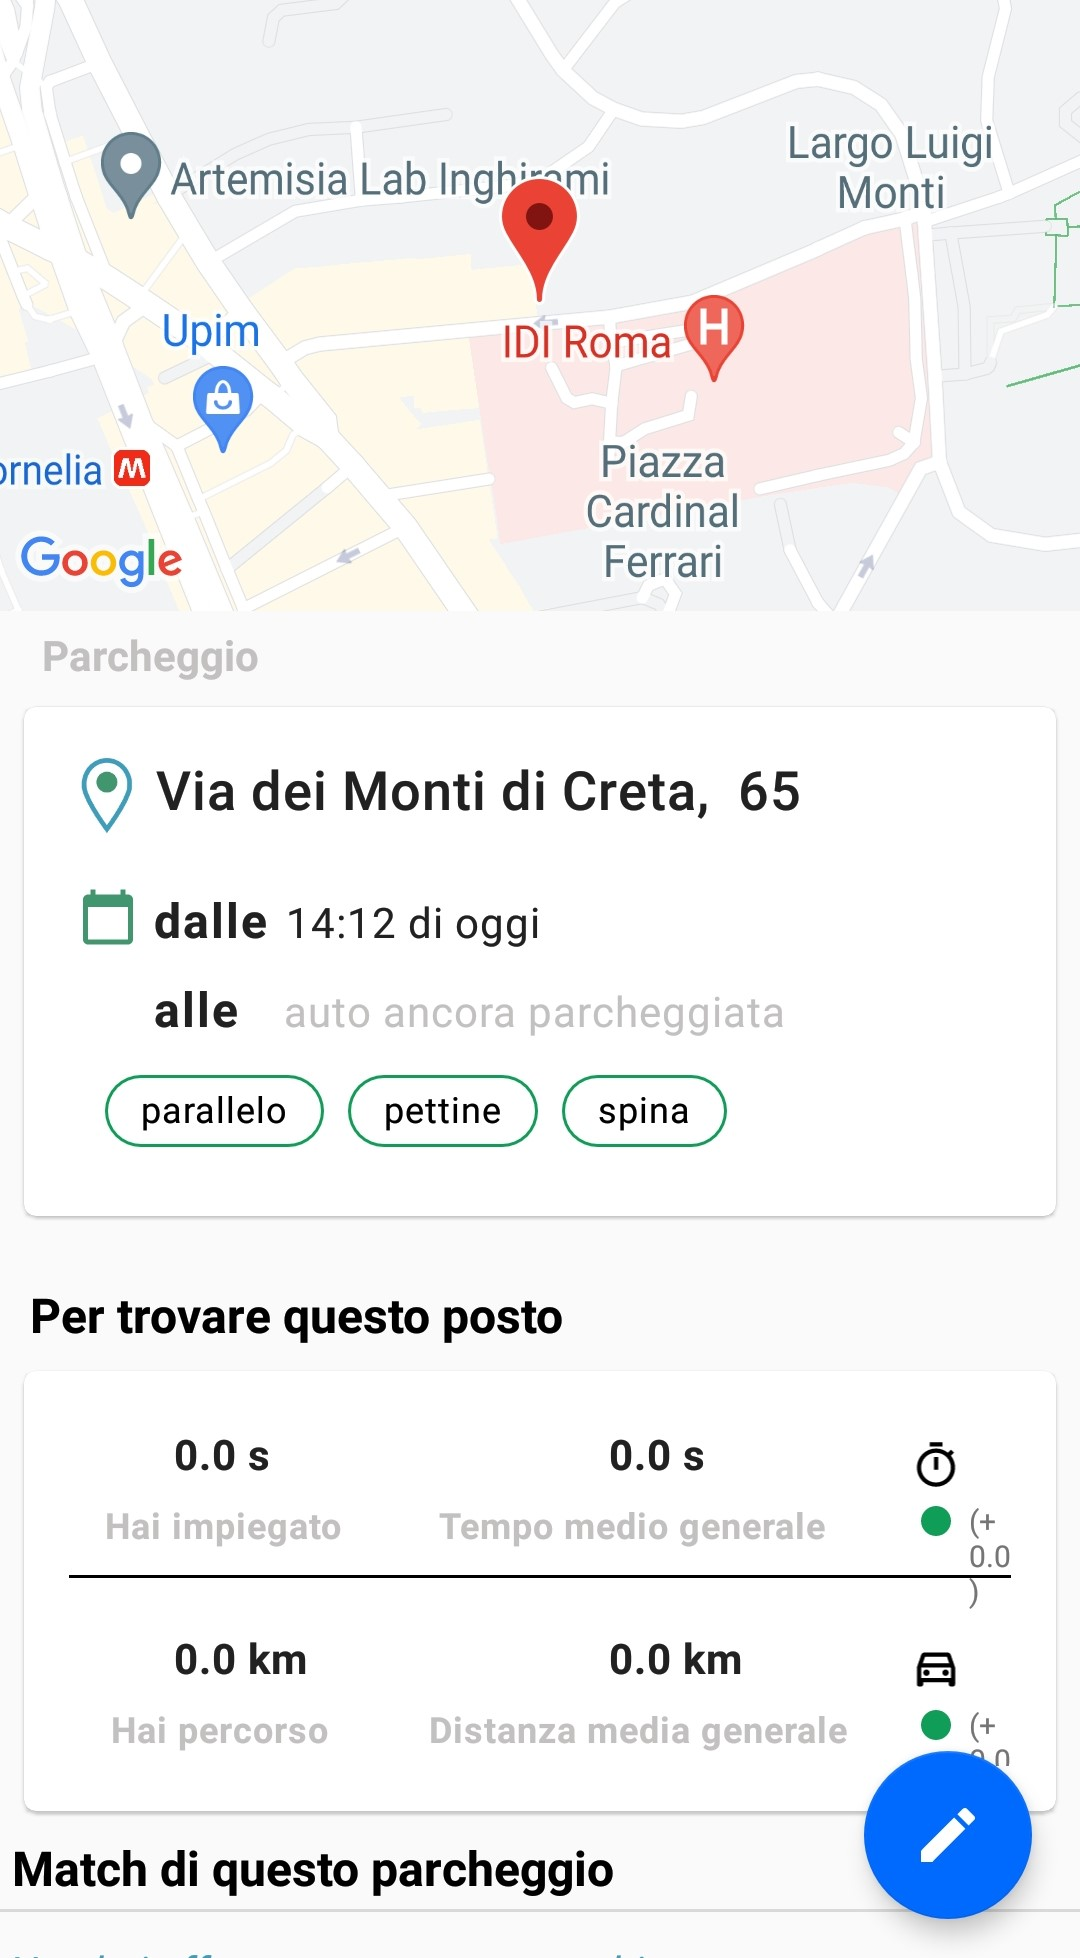
\includegraphics[width=6cm]{Floating_Action_Button.jpg}
\caption{Pagina dei dettagli di un parcheggio con
\texttt{FloatingActionButton}}
\end{figure}

È stata presa questa decisione in quanto, nei test effettuati, gli utenti navigavano nella pagina contenente i dettagli di un parcheggio cercando un modo per modificare l'indirizzo.

Il terzo problema è stato risolto rendendo modificabile l'indirizzo presente nel \texttt{ChangeParkPositionFragment}. In questa maniera l'utente è sempre al corrente del nuovo indirizzo del parcheggio, ma può cliccare su di esso per modificarlo tramite tastiera.

\begin{figure}[H]
\centering
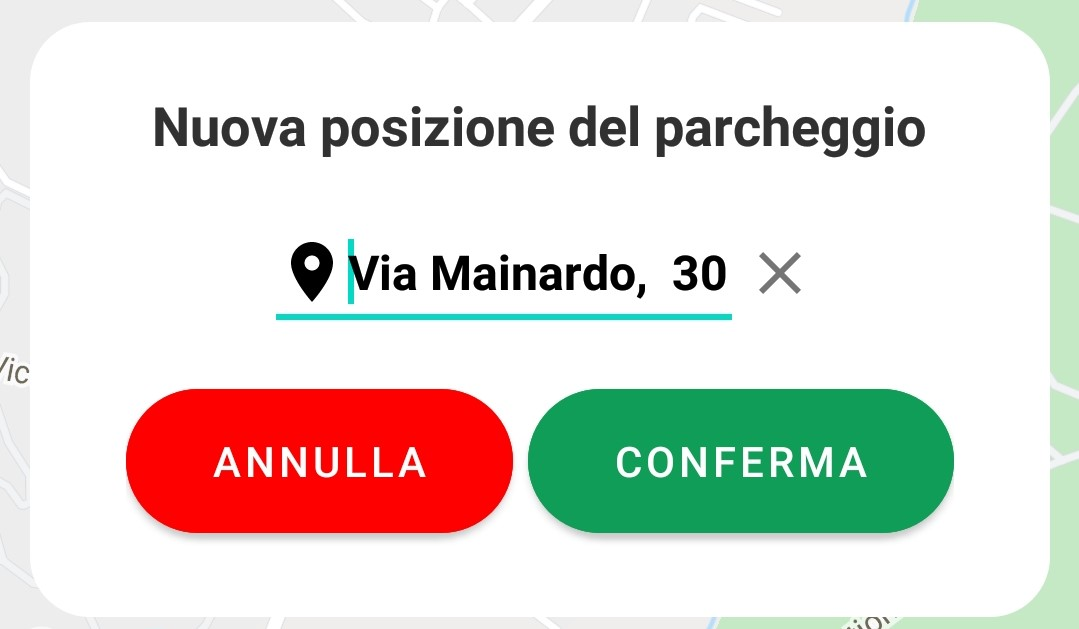
\includegraphics[width=6cm]{images/Editable_new_address.jpg}
\caption{\texttt{ChangeParkPositionFragment} con indirizzo modificabile}
\end{figure}

\hypertarget{test-1}{%
\subsubsection{Test}\label{test-1}}

Sono stati effettuati ulteriori test utilizzando la seconda iterazione dell'interfaccia e gli utenti sono riusciti a modificare il parcheggio utilizzando il \texttt{FloatingActionButton} nella pagina dei dettagli del parcheggio corrente.

Una volta entrati nella schermata per la modifica del parcheggio, gli utenti hanno spostato la mappa manualmente quando si chiedeva loro di modificare la posizione del parcheggio in una posizione molto vicina a quella attuale, mentre hanno utilizzato il campo di testo editabile quando è stato chiesto loro di modificare la posizione del parcheggio in una via più distante dalla posizione attuale, e quindi più difficile da trovare muovendo manualmente la mappa.

Non sono stati trovati ulteriori problemi di usabilità, e quindi l'interfaccia può essere considerata definitiva. 

\hypertarget{implementazione}{%
\chapter{Implementazione}\label{implementazione}}

In questo capitolo si discuteranno i dettagli implementativi di una funzionalità in particolare di quelle sviluppate. Si è scelta la funzionalità di aggiornamento della posizione del Taker in real-time sull'interfaccia mostrata al Giver.
\section{Aggiornamento posizione Taker in real-time}
Il flusso della funzionalità è stato descritto nella \autoref{aggiornamento-della-posizione-del-taker}.

\subsection{Invio periodico della posizione al server}\label{invio-periodico-posizione-taker}
Per ripetere un'azione in maniera periodica ogni $x$ secondi, all'interno del metodo \texttt{onCreateView()} del \texttt{MatchFoundFragment} viene inizializzato un oggetto \texttt{Runnable} il cui scopo è quello di eseguire la funzione per ottenere la posizione del Taker ed inviarla al server tramite una chiamata alle API.

Come è possibile vedere nel codice mostrato in  \autoref{inizializzazione-runnable}, il \texttt{Runnable} viene inserito all'interno di un \texttt{Handler}, e quindi eseguito immediatamente per la prima volta.

\begin{lstlisting}[caption=Inizializzazione del runnable,  label=inizializzazione-runnable]

takerPositionUpdateHandler = new Handler();
takerPositionUpdateRunnable = this::startTakerPositionUpdate;
takerPositionUpdateHandler.post(takerPositionUpdateRunnable);
\end{lstlisting}

L'effettivo codice che viene utilizzato dal \texttt{Runnable} per ottenere la posizione ed inviarla al server è incapsulato all'interno del metodo \texttt{startTakerPositionUpdate()} mostrato in \autoref{invio-posizione-taker}.

\begin{lstlisting}[caption=Metodo per l'invio della posizione del Taker al server,  label=invio-posizione-taker]
private void startTakerPositionUpdate() {
    FusedLocationProviderClient fusedLocationProviderClient = LocationServices.getFusedLocationProviderClient(app);
    if (ActivityCompat.checkSelfPermission(app.getApplicationContext(), Manifest.permission.ACCESS_FINE_LOCATION) != PackageManager.PERMISSION_GRANTED
            && ActivityCompat.checkSelfPermission(app.getApplicationContext(), Manifest.permission.ACCESS_COARSE_LOCATION) != PackageManager.PERMISSION_GRANTED) {
        return;
    }
    fusedLocationProviderClient.getLastLocation().addOnCompleteListener(task -> {
        if (task.getResult() != null) {
            MatchUtils.updateTakerPosition(app, new LatLng(task.getResult().getLatitude(), task.getResult().getLongitude()));
        }
        takerPositionUpdateHandler.postDelayed(takerPositionUpdateRunnable, LONG_TIMEOUT);
    });
}
\end{lstlisting}

Alla fine della chiamata API effettuata dal metodo, il \texttt{Runnable} viene aggiunto nuovamente all'\texttt{Handler} tramite il metodo \texttt{Handler.postDelayed}, che eseguirà il \texttt{Runnable} nuovamente dopo aver atteso un tempo specificato in \texttt{LONG\_TIMEOUT}, che in questo caso è di \texttt{5000ms}.

\begin{lstlisting}[caption=Body della chiamata alle API per l'aggiornamento della posizione del Taker, label=body-aggiornamento-posizione]
{
  "lat": 41.89891375106414,
  "lon": 12.3247983291,
  "schedule": "2020-05-14T12:12:58+02:00",
  "eta": 65
}
\end{lstlisting}

Nel \autoref{body-aggiornamento-posizione} viene mostrato il \texttt{body} della chiamata alle API che il Taker effettua per aggiornare la posizione al server. Il body è un oggetto json contenente le seguenti informazioni:
\begin{itemize}
\item
  \texttt{lat}: la latitudine del Taker;
\item
  \texttt{lon}: la longitudine del Taker;
\item
  \texttt{schedule}: un \texttt{timestamp} formattato come stringa, il quale fa riferimento al campo omonimo all'interno dell'oggetto Match documentato in \autoref{match}, che indica quando il Taker intende  occupare un posto;
\item
  \texttt{eta}: il tempo previsto, indicato in secondi, prima dell'incontro tra il Taker ed il Giver.
\end{itemize}

\subsection{Ricezione notifiche push}
Nella \autoref{invio-periodico-posizione-taker} si è discusso il modo in cui il client del Taker invia la posizione aggiornata al server. In questa sezione si parlerà invece del modo in cui il Giver ottiene la nuova posizione dal server e procede con l'aggiornamento sull'interfaccia. 

Come già accennato, l'informazione relativa alla posizione del Taker viene inviata al client del Giver tramite una notifica push, tramite il servizio \emph{Firebase Cloud Messaging} (\emph{FCM}).

Per configurare il client alla ricezione di notifiche da parte di questo servizio, viene creata una classe \texttt{NotificationService} che estende \texttt{FirebaseMessagingService}.

Come mostrato in \autoref{firebase-service-in-manifest}, il \texttt{Service} viene aggiunto al file \texttt{AndroidMainfest.xml} per rendere consapevole l'applicazione della sua esistenza, e quindi per permetterne il corretto funzionamento.

\begin{lstlisting}[caption=Aggiunta del \texttt{Service} all'interno del file \texttt{AndroidMainfest.xml}, label=firebase-service-in-manifest]
<service
    android:name=".services.NotificationService"
    android:exported="false">
    <intent-filter>
        <action android:name="com.google.firebase.MESSAGING_EVENT"/>
    </intent-filter>
</service>
\end{lstlisting}

Il primo passo per permettere la ricezione di notifiche push da parte
del client è quello di inviare al server il Token di registrazione generato dal \texttt{FCM SDK} all'avvio dell'applicazione, e relativo all'istanza dell'applicazione stessa. La conoscenza da parte del server di questo Token è di fondamentale per rendere possibile la comunicazione uno-ad-uno.

\begin{lstlisting}[caption=Invio del Token al server, label=invio-token]
@Override
public void onNewToken(@NonNull String s) {
    super.onNewToken(s);
    //API call to update the push notification token
    app.me(false, me -> {
        app.api().updatePushToken(s).enqueue(new Callback<String>() {
            @Override
            public void onResponse(Call<String> call, Response<String> response) {
                Log.d(TAG, "onResponse: " + response.body());
            }

            @Override
            public void onFailure(Call<String> call, Throwable t) {
                Log.e(TAG, "onFailure: " + t.getMessage());
            }
        });
    });
}
\end{lstlisting}

Come mostrato in \autoref{invio-token}, viene effettuato un \emph{override} del metodo \texttt{onNewToken}, il quale viene chiamato dal client ogni volta che il \texttt{FCM SDK} ne genera uno nuovo.

Il Token viene inviato al server all'interno del \texttt{body} della chiamata alle API con \texttt{endpoint "/me/push/tokens/"} e metodo \texttt{HTTP POST}.

Viene poi effettuato un \emph{override} del metodo \texttt{onMessageReceived} che viene chiamato ogni volta che il client riceve una notifica push dal server.

\begin{lstlisting}[caption=Override del metodo per gestire la ricezione di notifiche push, label=onMessageReceived]
@Override
public void onMessageReceived(@NonNull RemoteMessage remoteMessage) {
    super.onMessageReceived(remoteMessage);
    Map<String, String> data = remoteMessage.getData();
    if (data.get("lat") != null && data.get("lon") != null) {
        LatLng takerPosition = new LatLng(Double.parseDouble(data.get("lat")), Double.parseDouble(data.get("lon")));
        Intent intent = new Intent("TakerPosition");
        intent.putExtra("latLng", takerPosition);
        broadcaster.sendBroadcast(intent);
    }
}
\end{lstlisting}

All'interno di questo metodo viene creato un oggetto \texttt{LatLng} contenente le coordinate del Taker estratte dai campi \texttt{lat} e \texttt{lon} del messaggio della notifica.

L'oggetto contenente le coordinate viene inserito all'interno di un \texttt{Intent} che viene inviato al \texttt{LoacalBroadcastManager}.

\begin{lstlisting}[caption=Gestione dell'intent, label=notificationReceiver]
private final BroadcastReceiver notificationReceiver = new BroadcastReceiver() {
    @Override
    public void onReceive(Context context, Intent intent) {
        Log.d("NotificationDebug", "NotificationReceiver data: " + Objects.requireNonNull(intent.getExtras()).getParcelable("latLng"));
        LatLng takerPosition = Objects.requireNonNull(intent.getExtras()).getParcelable("latLng");
        if (takerPositionMarker != null) {
            MarkerAnimationUtils.animateMarkerToGB(takerPositionMarker, takerPosition, new LatLngInterpolator.Linear());
        }
    }
};
\end{lstlisting}

In \autoref{notificationReceiver} viene mostrato come viene gestita la ricezione dell'\texttt{Intent} inviato in \autoref{onMessageReceived}.

In particolare, viene estratto l'oggetto \texttt{LatLng} contenente le coordinate, e viene spostato il marker in tali coordinate mediante un'animazione fluida dalla durata di \texttt{5000ms}. \footnote{Animazione permessa dalla libreria raggiungibile al \href{https://gist.github.com/jcholin/a0afa38e606f9722680cbc25c3cea46b}{seguente link.}}

La durata dell'animazione è stata impostata a \texttt{5000ms} in quanto questo è il tempo che passa tra una notifica push e l'altra. In questo modo il cambio di posizione ottenuto durante le varie notifiche push ottenuto sarà il più fluido possibile. 
\chapter{Conclusioni}

\section{Sommario}

Nel \autoref{introduzione} sono stati analizzati gli obiettivi che l'applicazione su cui si è svolto il lavoro vuole risolvere, ed in che modo promette di farlo.

Nel \autoref{tecnologie-utilizzate} sono state mostrate le tecnologie utilizzate all'interno del tirocinio, insieme ai concetti fondamentali per lo sviluppo di applicazioni Android.

Nel \autoref{progettazione} è stata discussa la fase di progettazione della UI (User Interface) e della UX (User Experience). La prima è volta a comprendere come organizzare gli elementi mostrati sullo schermo in maniera da rendere l'applicazione facile da utilizzare; la seconda è volta a capire in che modo strutturare l'intero sistema per rendere l'esperienza che l'utente ha con quest'ultimo il più piacevole possibile.

Sono stati quindi mostrati i prototipi delle interfacce che sono state sviluppate, descrivendo le relative funzionalità, e sono stati documentati i test di usabilità effettuati, elencando i problemi individuati e le soluzioni che sono state proposte, fino all'arrivo di un'interfaccia completa.

Nel \autoref{implementazione} sono stati approfonditi i dettagli implementativi circa le interfacce e funzionalità progettate nel \autoref{progettazione}, mostrando le parti di codice significative che hanno portato alla realizzazione delle funzionalità desiderate.

Il tirocinante, alla fine del lavoro, ha maturato le seguenti capacità:
\begin{itemize}
    \item Progettazione di un prototipo di interfaccia;
    \item Implementazione di un'interfaccia all'interno di Android a partire da un prototipo;
    \item Sviluppo di funzionalità in ambito Android in linguaggio Java;
    \item Effettuare chiamate API e gestire le risposte.
\end{itemize}

\pagebreak
\section{Sviluppi Futuri}
Dall'inizio del tirocinio alla fine di quest'ultimo all'interno dell'applicazione sono state inserite numerose funzionalità, tuttavia l'applicazione è ancora nelle prime fasi di sviluppo e quindi sono molteplici quelle che ancora possono essere implementate.

Le funzionalità principali a mancare per quanto riguarda la gestione dei match sono:
\begin{itemize}
    \item La possibilità di un utente di cercare un posto in una zona differente da quella in cui si trova attualmente;
    \item La possibilità di un utente di cercare un posto in un orario differente da quello attuale, in modo da prenotarsi il posto per un momento futuro della giornata;
    \item La possibilità di un utente di essere Giver e Taker contemporaneamente.
\end{itemize}

A parte le prime due funzionalità che sono abbastanza autodescrittive, in questa sezione si descriveranno i dettagli e le complicazioni riguardanti la possibile implementazione della terza funzionalità.

Si ipotizzi che le prime due funzionalità elencate sopra già esistano all'interno dell'applicazione, e si ipotizzi la seguente situazione:
\begin{enumerate}
    \item Sia A un utente attualmente parcheggiato;
    \item A effettua un "Cerca posto" in un'altra zona;
\end{enumerate}

L'utente diventa quindi un Taker e raggiunge il Giver B associato per occupare il suo posto. Essendo l'utente A però parcheggiato, ed essendo egli un Taker, non può effettuare un "Lascia posto" prima di raggiungere l'utente B. 

Questo vuol dire che il posto da lui lasciato non verrà immediatamente occupato da un eventuale Giver C.

È possibile risolvere questo problema dissociando le azioni di "Cerca posto" e "Lascia posto", in modo che queste siano eseguibili indipendentemente l'una dall'altra.

Un utente A parcheggiato che intende effettuare un "Cerca posto", potrebbe quindi effettuare prima un "Lascia posto" per trovare un Taker B compatibile che occupi il suo attuale posto.
Effettuerà il "Cerca posto" nell'attesa che il Taker arrivi nella sua posizione, in modo da trovarsi già un utente Giver C compatibile. Una volta che il Taker B sia arrivato nella posizione dell'utente A e questi si siano scambiati i posti, l'utente A raggiungerà l'utente C per scambiare il posto auto con lui.



\backmatter
\phantomsection
\begin{thebibliography}{17}

\bibitem{istat-mobilita}
Sistema statistico nazionale Istituto nazionale di statistica 
\url{https://www.istat.it/storage/ASI/AnnuarioStatistico_2020/Asi_2020.pdf}

\bibitem{progetto-sparta}
Progetto SPARTA: ridurre l'inquinamento grazie allo smart parking e all'analisi del traffico.
\url{https://www.greenvulcano.com/it/progetto-sparta-ridurre-linquinamento-grazie-allo-smart-parking-e-allanalisi-del-traffico/}

\bibitem{smart-parking}
Smart parking: tutto ciò che bisogna sapere sul parcheggio intelligente
\url{https://www.backtowork24.com/news/smart-parking-tutto-cio-che-bisogna-sapere-sul-parcheggio-intelligente}

\bibitem{generocity}
GeneroCity \url{https://www.generocity.it/}

\bibitem{ui-ux-design-process}
A Step by Step Guide to UI/UX Design Process \url{https://aufaitux.com/blog/ui-ux-design-process/}

\bibitem{ux-design-process-steps}
The UX Design Process: Everything You Need to Know \url{https://xd.adobe.com/ideas/guides/ux-design-process-steps/}

\bibitem{test-usabilita}
Test di usabilità
\url{https://designers.italia.it/kit/test-usabilita/}

\bibitem{euristiche-nielsen}
Nielsen e le sue 10 euristiche
\url{https://www.far.unito.it/usabilita/cap5.htm}

\bibitem{activity}
Activity
\url{https://developer.android.com/reference/android/app/Activity}

\bibitem{activity-lifecycle}
Activity Lifecycle
\url{https://developer.android.com/guide/components/activities/activity-lifecycle}

\bibitem{fragments}
Fragments
\url{https://developer.android.com/guide/fragments}

\bibitem{fragment-lifecycle}
Fragment Lifecycle
\url{https://developer.android.com/guide/fragments/lifecycle}

\bibitem{intents}
Intents
\url{https://developer.android.com/guide/components/intents-filters}

\bibitem{services}
Services
\url{https://developer.android.com/guide/components/services}

\bibitem{what-is-restful-api}
What is RESTful API
\url{https://devdotcode.com/what-is-restful-api/}

\bibitem{rest-api-design}
REST API: Key Concepts, Best Practices, and Benefits
\url{https://www.altexsoft.com/blog/rest-api-design/}

\bibitem{wireframe}
Come creare un wireframe interattivo
\url{https://alfredoiannone.com/2018/05/02/come-creare-un-wireframe-interattivo/}

\bibitem{wireframe-kit}
Il modello di un’interfaccia e il Wireframe Kit
\url{https://design-docs-francescozaia.readthedocs.io/en/revisione-capitolo-ui/doc/user-interface/il-modello-di-un-interfaccia-e-il-wireframe-kit.html}

\bibitem{differenza-wireframe-prototipo}
Qual è la differenza tra Wireframe, Prototipo e Mockup?
\url{http://www.fabiomarasco.it/la-differenza-tra-wireframe-prototipo-e-mockup/}

\bibitem{framents-lifecycle-2}
Android Fragments: sperimentiamo il ciclo di vita
\url{https://www.devapp.it/wordpress/android-fragments-sperimentiamo-il-ciclo-di-vita/}

\bibitem{retrofit}
Using Retrofit 2.x as REST client
\url{https://www.vogella.com/tutorials/Retrofit/article.html}

\end{thebibliography}

\end{document}